\documentclass[PaulGanssle-Thesis.tex]{subfiles}

\begin{document}
\chapter{Low Field NMR}
\label{Chapter:NMR}
\section{Overview}
\label{nmr.overview}
Nuclear magnetic resonance is a tool with wide applicability across many disciplines in both industrial and research contexts. Traditional NMR experiments are performed using superconducting coils to generate magnetic fields which are both strong and homogeneous, which are generally used to perform either some chemical analysis, for tomographic imaging (generally of optically opaque media)\cite{Kumar1975,Kumar1975a,Mossle2006}, or both.\cite{Levitt2008}

The magnetic field plays two roles in an NMR experiment, it polarizes the spins (see \Cref{nmr.prepolarization} for more details), and it induces precession in spins aligned transverse to the field, at frequency $\omega_{0} = \gamma\mathbf{B_{0}}$, where $\gamma$ is the gyromagnetic ratio of the spin and $B_{0}$ is the bias field strength.\cite{Bloch1950,Hahn1950a} Most NMR experiments are detected using inductive coils, which detect the first time derivative of the magnetic flux through the coil, and as such the sensitivity of the detector is an increasing function of the frequency of the signal. As such, strong fields both increase the signal generated by the sample and increase the sensitivity of the detector.\cite{Savukov2007} As a consequence of the dependence of spin frequency on magnetic field strength, signal coherence - and as a consequence resolution - depends upon the homogeneity of the field.\cite{Bloom1955,hurlimann-jmr-2001}

Much work has been done on applications of NMR in situations wherein one or more of these constraints either must or can be relaxed. Generally speaking, the discipline of low-field NMR is concerned with NMR performed without employing superconducting magnets; this includes small-molecule NMR spectroscopy\cite{Moresi2003} performed using specially-constructed permanent magnets as well as \textit{ex-situ} NMR measurements such as those used in oil-well logging,\cite{kleinberg-cmr-2001,hurlimann-emr-2012} wherein measurements of relaxation and diffusion are performed in the gradient field generated by a single-sided NMR instrument\cite{single-sided-nmr,blumich-mri-mouse-1998,guthausen-jaocs-2004} (see \Cref{relaxometry} for further discussion of these techniques).

The use of various hyperpolarization techniques like spin-exchange optical pumping of noble gases,\cite{Walker1997,Goodson2002,Schroder2008} para-hydrogen induced polarization\cite{Theis2011,Lloyd2012} and dynamic nuclear polarization\cite{Maly2008,bentum-2011} allow the creation of highly polarized samples, generally far in excess of what can be achieved using the bias field for sample polarization; meanwhile the development of low-frequency magnetic field detectors such as Superconducting QUantum Interference Devices (SQUIDs)\cite{Webb1977,Meredith1973} or vapor cell magnetometers has dramatically increased detector sensitivity in low magnetic fields. The latter improvement has led to the development of ultra-low-field NMR and MRI, wherein detection takes place in Earth's magnetic field\cite{appelt-natphys-2006} or at even lower fields in magnetically shielded environments.\cite{Mossle2006,Ledbetter2011,Schwindt2004,Seltzer2004,Ledbetter2008}

\section{Sample Prepolarization}
\label{nmr.prepolarization}
\begin{wrapfigure}{L}{0.4\tw}
\vspace*{-0.5\lineheight}
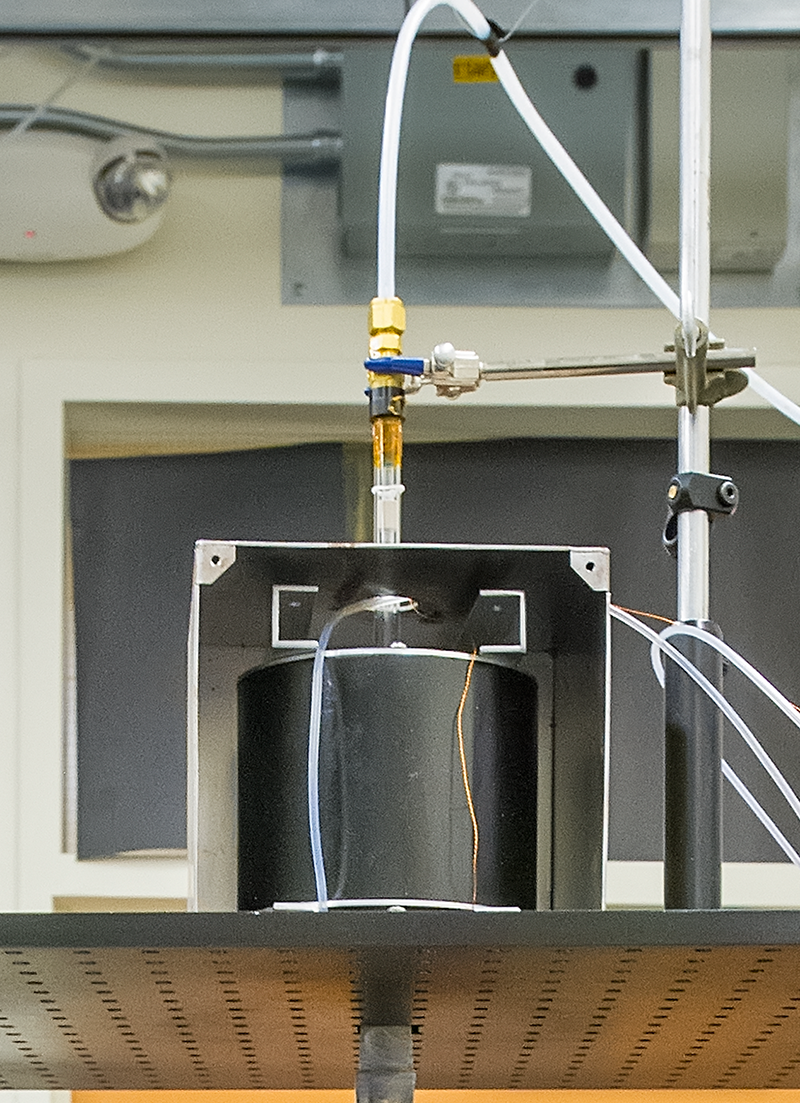
\includegraphics[width=0.4\tw]{figures/magnetometer/PolarizationRegionPhotoSmaller.png}
\caption{A photograph of the polarization region. The sample is shuttled up and down using the central vacuum and air lines, respectively.}
\vspace*{-2\lineheight}
\label{fig:PolarizationRegionPhoto}
\end{wrapfigure}
In NMR experiments, the quantity measured is the evolution of the net magnetization - which is a bulk property of an ensemble of spins. The net magnetization is directly related to the spin polarization, as each spin has a small magnetic dipole, which adds for coherent spins polarized in the same direction but subtracts for spins polarized in the opposite direction. The equilibrium spin polarization is given by Eqn. \ref{eqn:SpinBoltzmannDist}:

\begin{eqnarray}
\frac{P_{+} - P_{-}}{P_{+} + P_{-}} & = & \frac{1-e^{-\sfrac{\hbar\gamma B_0}{k_{B}T}}}{1 + e^{-\sfrac{\hbar\gamma B_0}{k_{B}T}}} \label{eqn:SpinBoltzmannDist}\\
 & = & \frac{e^{\sfrac{\hbar\gamma{}B_0}{2k_{B}T}}-e^{-\sfrac{\hbar\gamma B_0}{2k_{B}T}}}{e^{\sfrac{\hbar\gamma B_0}{2k_{B}T}} + e^{-\sfrac{\hbar\gamma B_0}{2k_{B}T}}} \\
 & = & \mathrm{tanh}\left(\frac{\hbar\gamma{}B_0}{2k_{B}T}\right).
\end{eqnarray}


For $\gamma B_0 \ll k_{B}T$, it is appropriate to use the first-order Taylor expansion of the $tanh$ function, giving an approximate bulk polarization of:

\begin{equation}
\frac{P_{+} - P_{-}}{P_{+} + P_{-}} \approx \frac{\hbar\gamma B_0}{2k_{B}T}.
\end{equation}

At high field, this produces small but noticeable polarization, so for protons at room temperature (taken here as \unit[298]{K}), where $\gamma_{H}$ = \unitfrac[267.513]{rad$\cdot$ MHz}{T}, spin polarization is $\approx$ \unitfrac[3.43]{ppm}{T}. At zero field, however, the spin polarization is also 0, and even if a several Gauss prepolarizing pulse were used (roughly the maximum value without magnetizing the shields), the polarization level would be \unitfrac[0.343]{ppb}{G}, a loss in 4 orders of magnitude of an already small signal.

The signals generated herein are generated using a prepolarizing permanent magnet of either \unit[1 or 2]{T}, which sits outside the outermost layer of magnetic shielding. Spins rest in the field for at least a few $\mathrm{T}_1$ periods before being shuttled to the lower-field detection region. Under otherwise adiabatic sample transfer (see Sec. \ref{nmr.pneumatic.adiabatic.transfer} for more details), spin polarization dies off roughly as the $\mathrm{T}_1$ of the sample during the transfer. For $T_1 \leq t_{shuttle}$, the loss in signal between the two regions is negligible. This does, however, add a $\mathrm{T}_1$ filter into the output experiment, rendering short-$\mathrm{T}_1$ components of the sample relaxation impossible (or at least difficult) to measure by this method.

This sample prepolarization method is useful because it allows each characteristic experimental field to be individually optimized: the field in which spins are detected needs to be extremely homogeneous, but not necessarily extremely strong when using a magnetometer, the field in which spins are polarized needs to be extremely strong, but not necessarily extremely homogeneous. This allows us to use a not-necessarily homogeneous field for polarization and a low field for detection - whereas when these are the same field, it must be both large and homogeneous (such as fields generated by certain superconducting magnet designs). 

While prepolarizing with an inhomogeneous field can lead to inhomogeneous polarization, once polarized, the spins will still evolve coherently in a homogeneous magnetic field. For bulk samples the signal will be proportional to the integral of the field over the entire sample - and thus a small relative drop in the field in parts of the gradient will lead to a small relative drop in overall signal but no distortion. For imaging, in the absence significant spin diffusion during the transfer period, inhomogeneous prepolarization can lead to some small signal strength distortions - which can likely be corrected for by mapping the polarization gradient using a known standard.

\section{J-coupling Spectroscopy}
\label{nmr.signal.jcoupling}
One of the most compelling applications of magnetometry to date is J-coupling spectroscopy, which is a technique for measuring the magnetic resonance spectrum of spins as they evolve in response to indirect spin-spin dipolar couplings (called \textit{J-couplings}).\cite{Zax1984,McDermott2002,appelt-natphys-2006} These couplings are mediated by hyperfine interactions between the nuclear spins and their local electronic environment and thus depend on many factors of the molecular configuration - bond angles and distances, connectivity and electronic structure. However, since they are a function only of spin-spin interactions, they are largely independent of the local magnetic field and are present even at zero field. This insight has formed the basis of a significant branch of our research agenda exploring the use of atomic magnetometers as detectors for J-spectroscopy at zero field.\cite{Ledbetter2009,Theis2012,Butler2013,Theis2013}

\subsection{Theory}
\label{nmr.jcoupling.theory}
The standard liquid-state NMR Hamiltonian for a multi-spins system is given in Eqn \ref{eqn:NMRHamiltonian}:\cite{Butler2013a}

\begin{equation}
\label{eqn:NMRHamiltonian}
H = \sum_{i}\sum_{j\neq{i}}J_{ij}\mathbf{I}_{i}\cdot\mathbf{I}_{j} + \sum_{i}\gamma_{i}\mathbf{B}\cdot\mathbf{I}_{i}
\end{equation}

When the local magnetic field $\mathbf{B} = 0$, only the  J-coupling Hamiltonian remains:

\begin{equation}
\label{eqn:JCouplingHamiltonian}
H_{J} = \sum_{i}\sum_{j}\mathbf{I}_{j}\cdot\mathbf{I}_{j}.
\end{equation}

This interaction is thus available even in the presence of zero magnetic field. Still, the form of the Hamiltonian presents potential problems for NMR signal detection, as the scalar operator $\mathbf{I}_{i}\cdot\mathbf{I}_{j} = I_{ix}I_{jx} + I_{iy}I_{jy} + I_{iz}I_{jz}$ is completely spatially isotropic and invariant to any spatial transformation such as rotations or mirror inversions. 

\begin{equation}
\label{eqn:InitialDensityMatrix}
\rho_{0} = \frac{\hbar \gamma B_{0}}{2k_{B}T}\left(\sum_{i}\mathbf{I}_{i}\right)
\end{equation}

And the time-evolution of the density matrix is given by the Louisville Equation (Eqn. \ref{eqn:QuantumLousivilleEquation}):

\begin{equation}
\label{eqn:QuantumLousivilleEquation}
\frac{\partial \rho}{\partial t} = -\frac{i}{\hbar}\left[H, \rho\right].
\end{equation}

Unfortunately, $\left[\rho_{0}, H_{J}\right] = 0$ (see Sec. \ref{proofs.qm.jcoupling.initialrhocommutation} for a detailed proof), and so thermal polarization is a stationary state of the Hamiltonian. This is true at high field as well, but at high field the $B_{0}$ field provides an a magnetically anisotropic environment, and changing the orientations of the spins relative to that environment are sufficient to see precession. The J-coupling Hamiltonian, on the other hand, is spatially isotropic, and depends only on the \textit{relative} orientations of the interacting spins - and as such, changing their direction has no effect on the evolution of the state. 

For two coupled spins $I_1$ and $I_2$ rotated relative to one another by angle $\theta$ in the $x-z$ plane defined as the plane normal to $I_{1}\times I_{2}$:

\begin{equation}
\label{eqn:TwoSpinsThetaRotation}
\rho_{0} = \frac{\hbar\gamma B_{0}}{2k_{B}T}\left[\frac{1 + \cos(\theta)}{2}(I_{1z} + I_{2z}) + \frac{1 - \cos(\theta)}{2}\left(I_{1z} - I_{2z}\right) + \sin(\theta)I_{2x}\right]
\end{equation}


\subsection{Application}
\label{nmr.jcoupling.application}
The detectable evolution under the J-coupling comes from the $I_{z}-S_{z}$ terms in the density matrix. These terms show up naturally in the initial density matrix of an ensemble of heteronuclear spins. For the two spin case, the initial polarization is given by:

\begin{equation}
\rho_{0}  =  \frac{\hbar\gamma_{I}B_0}{2k_{B}T}I_{z} + \frac{\hbar\gamma_{S}B_{0}}{2k_{B}T}S_{z}
\label{eqn:ISDensityMatrix}
\end{equation} 

Which can be rearranged into the relevant parallel and antiparallel components of the density matrix:
 
\begin{equation}
\rho_{0} = \frac{\hbar B_{0}\left(\gamma_{I} + \gamma_{S}\right)}{4k_{B}T}\left(I_{z} + S_{z}\right) + \frac{\hbar B_{0}\left(\gamma_{I}-\gamma_{S}\right)}{4k_{B}T}\left(I_{z} - S_{z}\right)
\label{eqn:ISDensityMatrix2}
\end{equation}

As has already been shown from theory section (Sec. \ref{nmr.jcoupling.theory}), only terms corresponding to $I_{z} - S_{z}$ will evolve under the J-coupling Hamiltonian. As can be seen from Eqn \ref{eqn:ISDensityMatrix2}, heteronuclei will have a natural polarization in both the parallel and antiparallel configurations, corresponding to Eqn \ref{eqn:ISPolarization}:

\begin{align}
\label{eqn:ISPolarization}
P_{\uparrow\downarrow} = \frac{\gamma_{I} - \gamma_{S}}{2\gamma_{I}} & & P_{\uparrow\uparrow} = \frac{\gamma_{I} + \gamma_{S}}{2\gamma_{I}}
\end{align}

For the case of carbon-hydrogen pairs, $\gamma_H \approx 4\gamma_C$, so $P_{\uparrow\downarrow} = \sfrac{3}{8}$, while $P_{\uparrow\uparrow} = \sfrac{5}{8}$, and so the signal can be increased if the spins can be pulsed out of phase of one another. This has the additional advantage of allowing the ``start point'' of the experiment to be determined by the pulse, ensuring a consistent phase between transients. In the case of carbon and hydrogen, the simple 4:1 ratio allows $I_{z} + S_{z}$ terms to be easily transformed into $I_{z} - S_{z}$ terms (and vice-versa) by applying a $4\pi_{x}$ pulse to the hydrogens, which corresponds to a $\pi$ pulse to the carbons. This is particularly convenient because it starts the spins aligned along the $z$ axis, which is the sensitive direction of the magnetometer. 

In the more general case, for a pulse about the $y$ axis of angle $\theta_{I} = \theta + \frac{\Delta}{2}$ on spins $I_{z}$ and angle $\theta_{S} = \theta + \frac{\Delta}{2}$ $^{[}$\footnote{From this definition $\Delta = \frac{\theta_{I}\gamma_{S}}{2\gamma_{I}}$.}$^{]}$ on the $S_z$ spins applied to spins initially aligned along $I_{z} + S_{z}$, the density matrix evolves in Eqn \ref{eqn:ISPulseEvolution}\footnote{A full proof for this assertion is found in Sec. \ref{proofs.qm.jcoupling.pulseapplied}}:

\begin{align}
\label{eqn:ISPulseEvolution}
\rho(\theta) = &  \cos\left(\sfrac{\Delta}{2}\right)\cos(\theta)\left(I_{z} + S_{z}\right) + \cos\left(\sfrac{\Delta}{2}\right)\sin\left(\theta\right)\left(I_{x} + S_{x}\right)\\
& + \sin\left(\sfrac{\Delta}{2}\right)\sin\left(\theta\right)\left(I_{z} - S_{z}\right) - \sin\left(\sfrac{\Delta}{2}\right)\left(I_{x}-S_{x}\right)
\end{align}

Both $I_{z} - S_{z}$ and $I_{x} - S_{x}$ represent evolving, singlet polarization, along different spatial axes under the zero-quantum coherences evolving under the J-coupling Hamiltonian, and they are maximized when $\Delta = n\pi$ for  $n \in \mathbbm{Z}$, and so the optimal pulse length on the $\mathbf{I}$ spins is:

\begin{align}
\theta_{I,op} & = \theta_{S,op} - n\pi \nonumber\\ 
& = \theta_{I,op}\left(\frac{\gamma_{S}}{\gamma_{I}}\right) - n\pi\nonumber \\
\label{eqn:ISpinTipAngleOptima}
& = \frac{n\pi}{1-\frac{\gamma_{S}}{\gamma_{I}}}
\end{align}

When using scalar magnetometers, only the $\vec{z}$ component of the magnetic field is measured, and so only the $I_{z} - S_{z}$ terms are detectable (see Sec. \ref{nmr.jcoupling.detection}), and so the signal is maximized when $n$ is chosen such that $\sfrac{n\pi}{1-\frac{\gamma_{S}}{\gamma_{I}}}$ is as close to an integer value as possible. Alternatively, a composite pulse sequence can be used to guarantee both that $\Delta = n\pi$ and that all the spins are aligned along $\vec{z}$, so long as pulses can be applied along arbitrary directions. The sequence consists of applying a pulse of angle $\sfrac{\theta_{S,OP}}{2}$ along $\vec{x}$, followed by a pulse of $\theta_{I} = \pi$ along the direction $\sfrac{\theta_{S,OP}}{2}$ of the $\vec{z}$ axis (i.e. $\left[0, -\sin\left(\sfrac{\theta_{S,OP}}{2}\right), \cos\left(\sfrac{\theta_{S,OP}}{2}\right)\right]$), and finally a pulse along $\vec{x}$ of angle $-\sfrac{\theta_{S,OP}}{2}$.

The primary downside of this pulse sequence is the difficulty of applying pulses along an arbitrary direction. At high field, this is not as much of a problem, because in the rotating frame, phase shifting an RF signal corresponds to changing the direction of the pulse. At zero field, however, spins are not precessing about a large bias field, and so the pulse direction corresponds to a physical direction - in practice, this means that a linear combination of DC pulse coils must be used to apply pulses along an arbitrary direction. This can be complicated by differences in the response of each coil and potential digitization of potential output values. The pulses may need to be re-calibrated as a function of direction, and so it is likely less useful to use such a pulse sequence except in circumstances where pulse error due to gyromagnetic ratio mismatch are very large. For the most common case - hydrogen and carbon, $\sfrac{\gamma_{^{1}H}}{\gamma_{^{13}C}} = 3.9760836$. If a simple $4\pi$ pulse is applied to the hydrogen spins, the resulting pulse error is \unit[6]{mrad}. Each pulse of $\Delta = \pi$ corresponds to $\theta_{I} = \sfrac{1}{1-\frac{\gamma_{S}}{\gamma_{I}}}$, which is \unit[1.336$\pi$]{rad}, representing a pulse error of \unit[336]{mrad} away from ideal. However, on pulses of $\Delta = 3n\pi$, the pulse error is \unit[25.04$n$]{mrad}. For arbitrary $\gamma_{S}$ and $\gamma_{I}$, the optimal pulse time can be found iteratively:

\begin{equation}
\label{eqn:JcouplingOptimalNIteration}
n_i = n_{i-1}\mathrm{round}\left(\left|\mathrm{round}\left(\frac{n_{i-1}}{1-\frac{\gamma_{S}}{\gamma_{I}}}\right) - \frac{n_{i-1}}{1-\frac{\gamma_{S}}{\gamma_{I}}}\right|^{-1}\right)
\end{equation}

Starting with $n_0$ = 1 and $i > 0$. As this is an iterative product of increasing size (as the residuals get smaller $n_{i}$ gets larger), the optimal choice of $i$ is likely going to be fairly low, as errors in the pulse calibration are likely to swamp any gains from increasing optimality of pulses. For the $^{13}C-^{1}H$, $n_{i\in[0,4]}$ = (1, 3, 372, 107136, 98672256, 189944092800), corresponding to pulse errors of \unit[(1056, 25.2, 10.9, 3.41, 1.63, 0.575)]{mrad}. For a $^{15}N$-$^{1}H$ system, the first 3 terms are $n_{i\in[0,2]}$ = (1, 9, 579) corresponding to residuals of \unit[(354.5, 48.9, 13.8)]{mrad}. For these systems, using $n_{i} = 1$, as it represents at most a 2.5\% and 4.9\% drop in overall signal (to some extent this is mitigated by the fact that anti-parallel terms occur in the thermal distribution of heteronuclei, and so some signal is present even with no pulse). For a $^{13}C-^{15}N$ system, however, the first 4 terms are: $n_{i\in[0,3]}$ = (1, 3, 21, 630), which correspond to residuals of \unit[(903, 434, 106, 48.6)]{mrad}. As such, even the $n_{2}$ term represents a 10\% drop in signal. In a case such as this, it may be preferable to use a composite pulse sequence to prepare the initial state.

\subsection{Zero-Quantum Subspace}
\label{nmr.signal.jcoupling.zq}
Evolution under the J-coupling Hamiltonian takes place in the zero-quantum subspace - which consists of terms corresponding to terms with no change in total spin angular momentum. This can be easily demonstrated in the two-spin case, where the zero-quantum subspace terms correspond to $I_{+}S_{-}$ and $I_{-}S_{+}$, which represent coherences between states of the form $\left|\uparrow\downarrow\right\rangle$ and $\left|\downarrow\uparrow\right\rangle$; in this special case, the 2$\times$2 zero-quantum subspace can be treated as a single pseudo-spin, with axes $ZQ_{x}$, $ZQ_{y}$ and $ZQ_{z}$, which can be expressed as linear combinations of the appropriate single-spin operators.

\subsection{Detectable Coherences}
\label{nmr.jcoupling.detection}
While precession under the J-coupling Hamiltonian is necessary to observe J-spectroscopy, it is not alone sufficient, as coherences must also produce a net magnetic dipole. The general quantum mechanical observable associated with the magnetic dipoles generated by an ensemble of polarized spins is given by Eqn. \ref{eqn:GeneralDipoleObservable}:

\begin{equation}
\label{eqn:GeneralDipoleObservable}
\mu_{z} = \hbar\gamma_{I}\sum_{i}I_{iz} 
\end{equation}

Taking as an example the two-spin case, the spins are initialized along $ZQ_{z}$ ($ZQ_{z} = I_z - S_z$), and the Hamiltonian lies along the $ZQ_{x}$ axis, inducing the spins to precess in the $ZQ_{y} - ZQ_{z}$ plane:

\begin{align}
\label{eqn:JCouplingPrecession}
\rho(t) & = e^{-iJ_{IS}(I_{x}S_{x} + I_{y}S_{y})t}(I_{z} - S_{z})e^{iJ_{IS}(I_{x}S_{x} + I_{y}S_{y})t} \nonumber \\
 &= \mathrm{cos}(J_{IS}t)(I_{z} - S_{z}) - \mathrm{sin}(J_{IS}t)(I_{x}S_{y} - I_{y}S_{x})
\end{align}

The magnetometer signal will then be given by the expectation value of the dipole operator, $\langle \mu_{z} \rangle$. The expectation value of an operator is equivalent to the trace of that operator operated on the density matrix (Eqn. \ref{eqn:ExpectationValueFromDensityMatrix}):

\begin{equation}
\label{eqn:ExpectationValueFromDensityMatrix}
\langle A\rangle(t) = \mathrm{Tr}\left[\rho(t)A\right]
\end{equation}

This can be written as:

\begin{align}
\left\langle\mu_{z}\right\rangle = & \hbar\cdot\mathrm{Tr}\left[cos(J_{IS}t)(\gamma_{I}I_{z} + \gamma_{S}S_{z})(I_{z} - S_{z})\right.\nonumber \\
& \left. - \sin(J_{IS}t)(\gamma_{I}I_{z} + \gamma_{S}S_{z})(I_{x}S_{y} - I_{y}S_{x}) \right]
\end{align}

And because traces are linear functionals (i.e. $Tr(aA + bB) = aTr(A) + bTr(B)$), this can be split up into its constituent parts:

\begin{equation}
\left\langle\mu_{z}\right\rangle(t) = \hbar\cos\left(J_{IS}t\right)\mathrm{Tr}\left[\mu_{z}\left(I_{z} - S_{z}\right)\right] - \hbar\sin\left(J_{IS}t\right)\mathrm{Tr}\left[\mu_{z}\left(I_{x}S_{y} - I_{y}S_{x}\right)\right]
\end{equation}

The magnetization from the $ZQ_{z}$ term is then:

\begin{equation}
\left\langle\mu_{z,ZQ_{z}}\right\rangle(t) = \cos(J_{IS}t)\mathrm{Tr}\left[(\gamma_{I}I_{z} + \gamma_{S}S_{z})(I_{z}-S_{z})\right]
\end{equation}

And the magnetization from the $ZQ_{y}$ term is:

\begin{equation}
\left\langle\mu_{z,ZQ_{y}}\right\rangle(t) = -\sin(J_{IS}t)\mathrm{Tr}\left[(\gamma_{I}I_{z} + \gamma_{S}S_{z})(I_{x}S_{y}-I_{y}S_{x})\right]
\end{equation}

The value of the trace can be calculated from the following properties of the spin operators:

\begin{equation}
\label{eqn:SpinOpsIdentity}
I_{x}^2 = I_{y}^2 = I_{z}^2 = \mathbbm{1} 
\end{equation}

\begin{equation}
Tr(I_{x}) = Tr(I_{y}) = Tr(I_{z}) = 0
\label{eqn:SpinOpsTraceless}
\end{equation}

\begin{equation}
\label{eqn:SpinOpsTensors}
I_{i}S_{n} = \sigma_{i}\otimes\sigma_{n}
\end{equation}

\begin{equation}
\label{eqn:TraceTensors}
Tr(A\otimes B) = Tr(A)Tr(B)
\end{equation} 

From Eqns \ref{eqn:SpinOpsTensors} and \ref{eqn:TraceTensors}, we can separate the traces of heteronuclear products to the products of the traces of their homonuclear terms (e.g. $\mathrm{Tr}(I_{x}S_{x}) = \mathrm{Tr}(I_{x})\mathrm{Tr}(S_{x})$):

\begin{equation}
\label{eqn:DetectionOperatorZQZ1}
\left\langle\mu_{z,ZQ_{z}}\right\rangle(t) = \hbar\cos(J_{IS}t)\left[\mathrm{Tr}(\gamma_{I}I_{z}^2) - \mathrm{Tr}(\gamma_{S}S_{z}^2) - \mathrm{Tr}(I_{z})\mathrm{Tr}(S_{z}) + \mathrm{Tr}(I_{z})\mathrm{Tr}(S_{z})\right]
\end{equation}

\begin{align}
\left\langle\mu_{z,ZQ_{y}}\right\rangle(t) & = & -\hbar\sin(J_{IS}t)\left[\gamma_{I}\mathrm{Tr}(I_{z}I_{x})\mathrm{Tr}(S_{y}) \right. & - & \gamma_{I}\mathrm{Tr}(I_{z}I_{y})\mathrm{Tr}(S_{x}) \\
& &+ \gamma_{S}\mathrm{Tr}(I_{x})\mathrm{Tr}(S_{z}S_{y}) &-&\left. \gamma_{S}\mathrm{Tr}(I_{y})\mathrm{Tr}(S_{z}S_{x})\right]
\label{eqn:DetectionOperatorZQY1}
\end{align}

And from Eqn. \ref{eqn:SpinOpsTraceless}, all terms corresponding to the trace of a single spin operator (e.g. $S_z$, $I_x$) are 0, while squared spin operators are 1, per Eqn. \ref{eqn:SpinOpsIdentity}. The trace of two-spin mixed operators (e.g. $I_{x}I_{y}$) need not be calculated, as in these cases they are always paired with a a lone heteronuclear term. Plugging this in to Eqn. \ref{eqn:DetectionOperatorZQY1}, we find that the $ZQ_{y}$ term gives no detectable magnetization:

\begin{equation}
\label{eqn:DetectionOperatorZQY2}
\left\langle\mu_{z, ZQ_{y}}\right\rangle(t) = 0,
\end{equation}

and so only magnetization from the $ZQ_{z}$ term are detectable:

\begin{equation}
\label{eqn:DetectionOperatorTwoSpinFinal}
\left\langle\mu_{z}\right\rangle(t) = \cos(J_{IS}t)(\gamma_{I} - \gamma_{S}).
\end{equation}

\section{Magnetization Detection}
\label{nmr.signal.magnetization}
In many instances, rather than directly observe the spectral characteristics of the samples, it is preferable to look at the level of bulk magnetization of the sample - this is particularly true in experiments performed in an indirect dimension (see Sec. \ref{nmr.indirect}). The magnetization is simply a function of the spin polarization and gyromagnetic ratio and shows up on the a simple DC level on the magnetometer. However, the presence of \textit{any} magnetic field can cause a shift in the magnetometer signal, as can drift and noise - which is particularly high close to DC due to the presence of $\sfrac{1}{f}$ noise, and discrete noise sources from physical jostling of the instrument. An additional problem is that the sample magnetization decays over time as the spins relax to their non-polarized state, and as such have some low-frequency characteristics themselves beyond a simple DC offset. A proper measurement of the magnetization can be made by taking advantage of the fact that ensembles of spins react to magnetic pulses, while bias offsets and noise are invariant under such transforms. This allows one to design a pulse sequence which measures only sample magnetization and filter out other sources of magnetic field.

\subsection{$\pi$ Train}
\label{nmr.signal.magnetization.pitrain}
\begin{figure}[h!]
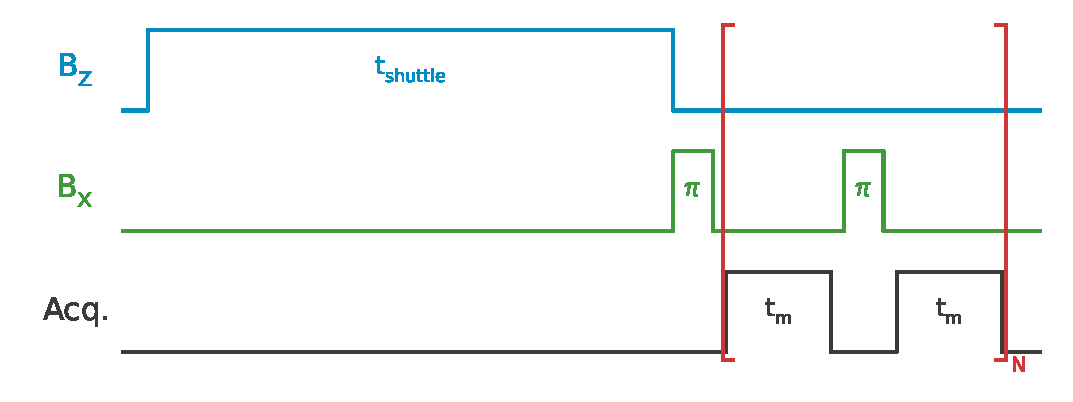
\includegraphics[width=\tw]{figures/relaxometry/acq_sequence_diagram.eps}
\caption{A magnetization detection sequence using a $\pi$ train along a single direction. A strong bias offset field is applied during the shuttling time to ensure an adiabatic transfer of magnetization.}
\label{fig:PiTrainDetection}
\end{figure}
The simplest and most common pulse sequence for the measurement of bulk sample magnetization is the application of a train of $\pi$ pulses transverse to the direction of initial polarization. This should invert the signal magnetization, and the change in DC level in response to a pulse corresponds to the signal magnetization - as other sources of magnetic field should be invariant under pulses, the difference in signal is

\begin{equation}
\Delta B = (B_{s} + B_{off}) - (-B_{s} + B_{off}) = 2B_{s},
\end{equation}

where $B_{s}$ is the field generated by the sample and $B_{off}$ is the field represented by any local fields which vary slowly with respect to the pulse time. Repeating this in a train of $\pi$ pulses separated by time $\tau$ should create signal which looks like a decaying square wave (as can be seen in Fig. \ref{fig:PiTrainDetection}). In a sense, this is similar to maximally-aliased version of the resonance condition present in a normal NMR experiment, where the observed effective frequency of oscillation is reduced to $\omega_0\sfrac{t_p}{t_p+\tau}$. One advantage of this method is that the inhomogeneous broadening induced by the pulses scales with $t_p$, while the relaxation will mostly scale with $\tau$, so a typical case of $t_p$ = \unit[100]{$\mu$s}, $\tau$ = \unit[50]{ms} and $\mathrm{T}_{2}$ = \unit[3]{s}, using the very inhomogeneous small pulsing coils (see Sec. \ref{nmr.pulsecoil.designs}), with a linewidth of \unit[2]{Hz} corresponding to a $T_{2}^{\mathbf{*}}$ of \unit[159]{ms}. The effective $T_{2}^{\mathbf{*}}$ from inhomogeneous broadening from the pulses is \unit[79]{s}, and so the pulse homogeneity does not play much role in the relaxation.

\begin{figure}[h!]
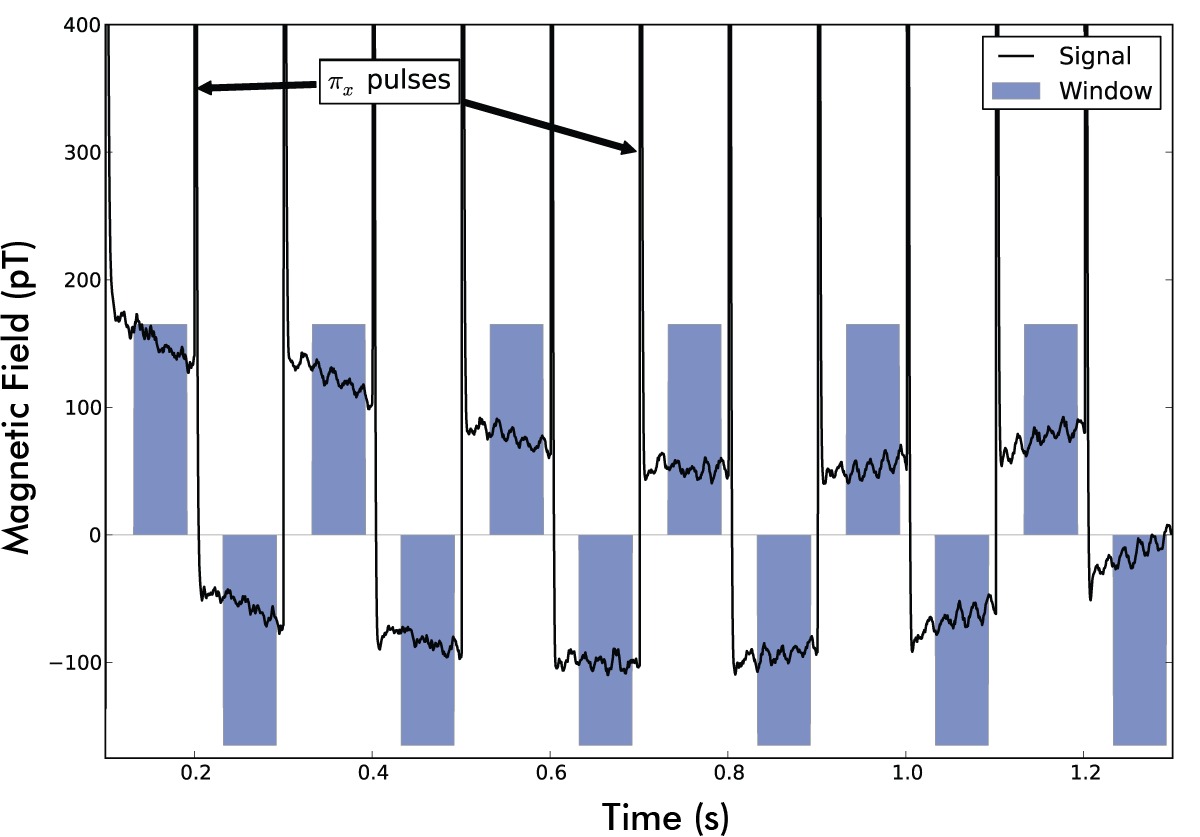
\includegraphics[width=\tw]{figures/relaxometry/12-07-17-WaterFIDFirst.png}
\caption{Direct dimension signal of water acquired using a $\pi$ train. The sample magnetization is determined from the change in the magnetic field between positive and negative ``window'' periods.}
\label{fig:PiTrainData}
\end{figure}


\subsubsection{Multiphase $\pi$ Trains}
\label{nmr.signal.magnetization.pitrain.variations}
Despite the simplicity of the 1$^{\textrm{st}}$ order effect - spin flipping - there are many variations available on the pulse sequence presented in Fig. \ref{fig:PiTrainDetection}, all of which can have different effects on different systems. The simplest variation is the use of pulses along $\vec{y}$, or indeed along any arbitrary phase $\vec{u}$ in the transverse plane. The main effect would be identical, but consider the case of a small, static bias offset magnetic field field along an arbitrary direction $\vec{v}$ that has been inadequately shimmed out. The effect of a train of evenly-spaced $\pi$ pulses along $x$ is:

\begin{align}
\label{eqn:PiXPulseEffect}
I_{x} & \rightarrow \phantom{-}I_{x} \nonumber\\
I_{y} & \rightarrow -I_{y}  \\
I_{z} & \rightarrow -I_{z} \nonumber
\end{align}

This is equivalent to a mirror reflection in both $\vec{y}$ and $\vec{z}$, which induces a series of spin echoes of the component of magnetization along $\vec{y}$ and $\vec{z}$, and the only remaining bias offset fields effectively felt by the spins are the fields along $\vec{x}$. This can be quite useful for removing persistent bias offset fields, as it allows each of the three axes to be addressed individually. Since the detection takes place along the longitudinal axis, applying a ``$\pi$ train'' along $\vec{z}$ is still possible, using the sequence $\frac{\pi}{2}_{x}-\pi_{z}-\frac{\pi}{2}_{x}$, which has the effect:

\begin{align*}
\label{eqn:PiZPulseEffect}
      && \specialcell{\hfill{}\left(\frac{\pi}{2}\right)_{x}\hfill{}} &&                  && \specialcell{\hfill{}\pi_{z}\hfill{}}  &&                  && \specialcell{\hfill{}\left(\frac{\pi}{2}\right)_{x}\hfill{}} &&& \\
I_{x} && \xrightarrow{\hspace*{2cm}}                                && \phantom{-}I_{x} && \xrightarrow{\hspace*{2cm}}          && -I_{x}           && \xrightarrow{\hspace*{2cm}}     && -I_{x}           &\\
I_{y} && \xrightarrow{\hspace*{2cm}}                                && -I_{z}           && \xrightarrow{\hspace*{2cm}}          && -I{z}            && \xrightarrow{\hspace*{2cm}}     && -I_{y}           & \\
I_{z} && \xrightarrow{\hspace*{2cm}}                                && -I_{y}           && \xrightarrow{\hspace*{2cm}}          && \phantom{-}I_{y} && \xrightarrow{\hspace*{2cm}}     && \phantom{-}I_{z} &                                    
\end{align*}

The downside to these pulses, however, is that it takes $\approx 2 t_{\pi}$ rather than $t_{\pi}$, but this is generally not particularly limiting, as the dead time of the magnetometer response is often substantially longer than the pulses themselves. The spin-echo generating properties of $\pi$ trains can also be used to greater effect by alternating the phases of the pulses at each pulse. For a $\pi_{x}-\tau-\pi_{y}-\tau$ sequence, the $\vec{y}$ and $\vec{z}$ components of the magnetization refocus at $2n\tau$. The $\vec{x}$ magnetization, however, refocus on $4n\tau$, because the first $\pi_{y}$ pulse does not occur until $2\tau$ after the spins begin to evolve. Additionally, the symmetry of the sequence allows the alternating $\pi$ pulses to correct the errors in the pulses of their complement as well, as the pulse errors are refocused as well:

\begin{equation}
I_{z} \xrightarrow{\pi_{x} + \varepsilon_{x}} -I_{z}\cos\left(\varepsilon_{x}\right)-I_{x}\sin\left(\varepsilon_{x}\right)\xrightarrow{\pi_{y}}I_{z}\cos\left(\varepsilon_{x}\right) + I_{x}\sin\left(\varepsilon_{x}\right) \xrightarrow{\pi_{x}+\varepsilon_{x}} -I_{z}
\label{eqn:PulseErrorCorrection}
\end{equation}

As can be seen in Eqn. \ref{eqn:PulseErrorCorrection}, error along the $\pi_{x}$ direction is corrected on every other pulse by the spin echo property of the $\pi_{y}$ pulse. When there are errors on both the $\pi_{x}$ and $\pi_{y}$ pulses, alternating the pulses partially corrects the pulses in the perpendicular direction. This follows a four-pulse series, with the residual error for $\varepsilon_{x},\varepsilon_{y}\ll 1$ after the 4$^{th}$ pulse given by:

\begin{equation}
\theta_{4} \approx 1 - \frac{\varepsilon_{x}^{4}\varepsilon_{y}^2 + \varepsilon_{x}^{2}\varepsilon_{y}^{4}}{8}
\end{equation}

And the residual error given by the 4$n^\textrm{th}$ pulse is:

\begin{equation}
\theta_{4n} \approx \left(1-\frac{\varepsilon_{x}^4\varepsilon_{y}^2 - \varepsilon_{y}^4\varepsilon_{x}^2}{8}\right)^{n^2} 
\end{equation}

And given that $\varepsilon_{x},\varepsilon_{y}\ll1$, this can be truncated at the 1st term:

\begin{equation}
\theta_{4n} \approx 1-n^2\left(\frac{\varepsilon_{x}^4\varepsilon_{y}^2 - \varepsilon_{y}^4\varepsilon_{x}^2}{8}\right)
\end{equation}

This can be compared to the error from a simple $\pi$ train, which scales linearly with $\varepsilon$. One thing to note, however, is that since the error correction takes place over the course of 4 pulses, the shot-to-shot error will still be on the order of $\varepsilon_{x}$ and $\varepsilon_{y}$. Using a fairly consistent pulse circuit, it is likely that the pulse error will be limited by the clock speed of the pulse controller. For a 100 MHz clock, the minimum pulse resolution is \unit[10]{ns}. For \unit[0.5]{G} pulses on protons, that corresponds to $\varepsilon =$ \unit[6.69$\cdot 10^{-5}$]{rad}, and so generally even a single-phase $\pi$-train does not introduce significant angular error due to pulse imperfections - though benefits can still possibly be gained by correcting for a shifting bias offset field. 

\subsubsection{Heteronuclear Magnetization}
\label{nmr.signal.magnetization.heteronuclei}
The simple and even multi-phase $\pi$ train methods of magnetization detection work only when the spins all have the same gyromagnetic ratio (and thus the same $\pi$ pulse duration). This is not the case in heteronuclear ensembles. While it may be possible to measure the J-spectrum, it is sometimes preferable to make a simple measurement of the magnetization, at least for testing purposes. For two nuclei, this can be accomplished easily with a simple composite pulse:

\begin{equation}
\label{eqn:HeteronuclearMagnetizationDetectionPulse}
\tfrac{\pi}{2}_{x, I} - \pi_{y,S} - \tfrac{\pi}{2}_{x,I}
\end{equation}

This works the same way as the error correcting pulses above, wherein the symmetry about the $\pi_{y}$ pulse cancels out any evolution about the $\vec{x}$ axis in the $\mathbf{S}$ spin, and since the $\mathbf{I}$ spins are along $\vec{y}$ when the pulse is applied, they are unaffected by the $\pi_{y}$ pulse. This is effectively the inverse of the composite J pulse described in Sec. \ref{nmr.jcoupling.application}, which attempts to invert the spins relative to one another, whereas this attempts to prevent them from dephasing while inverting their direction. This method is not simply generalized to higher numbers of nuclei, which should be taken on a case-by-case basis, taking into account the relative gyromagnetic ratios of the spins.

\subsection{Quadrature Signal Detection}
\label{nmr.signal.magnetization.quadrature}
While a $\pi$ train is sufficient for most experiments measuring only bulk sample magnetization, it measures only the scalar $\vec{z}$ magnetization of the sample and discards the information along $\vec{x}$ and $\vec{y}$ directions. This can be occasionally be useful information, particularly when acquiring free-induction decays in an indirect dimension. Take, for example, the signal acquired after the sequence detailed in Fig. \ref{fig:IndirectFIDSequence}:
\begin{figure}[ht!]
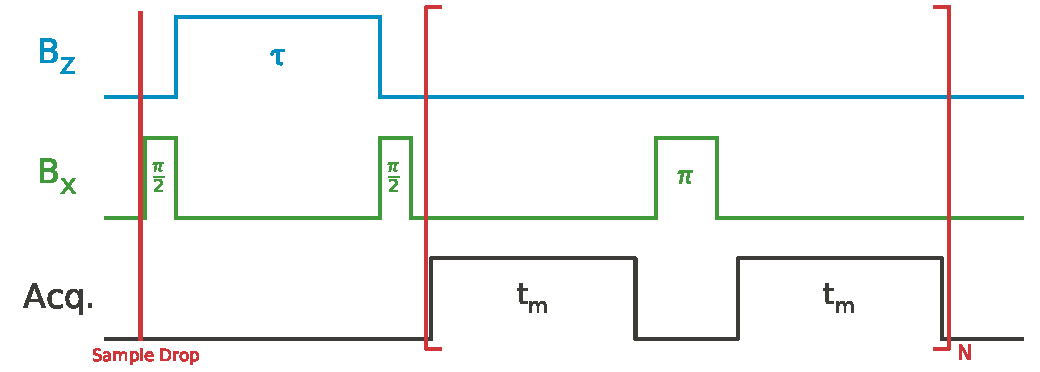
\includegraphics[width=\tw]{figures/relaxometry/fid_acq_sequence_diagram.pdf}
\caption{A sequence for acquiring FIDs in the indirect dimension.}
\label{fig:IndirectFIDSequence}
\end{figure}
The spins are tipped along $\vec{y}$ and allowed to precess for time $\tau$, resulting in the state:

\begin{equation}
\label{eqn:FIDIndirectDM}
\rho(\tau) = I_{y}\cos(\gamma_{I}B_{Z}\tau) - I_{x}\sin(\gamma_{I}B_{z}\tau) 
\end{equation}

After a second $\frac{\pi}{2}_{x}$ pulse, the spins are in the state:

\begin{equation*}
\rho_D(\tau) = -I_{z}\cos(\gamma_{I}B_{Z}\tau) - I_{x}\sin(\gamma_{I}B_{z}\tau)
\end{equation*}

If the standard pulse sequence is used, the signal will be $S(\tau) = \cos(\gamma_{I}B_{Z}\tau)$, which throws away the imaginary channel entirely - roughly half the signal. There are two ways to acquire the imaginary channel - one is to repeat the measurement, but instead replacing the second pulse with a $\frac{\pi}{2}_{-y}$ pulse. However, when the detection region is at zero field, since the remaining transverse component does not evolve except under the pulses, the imaginary channel can be also be acquired in a single acquisition by switching to the pulse sequence shown in Fig \ref{fig:QuadraturePulseSequence}:
\begin{figure}[ht!]
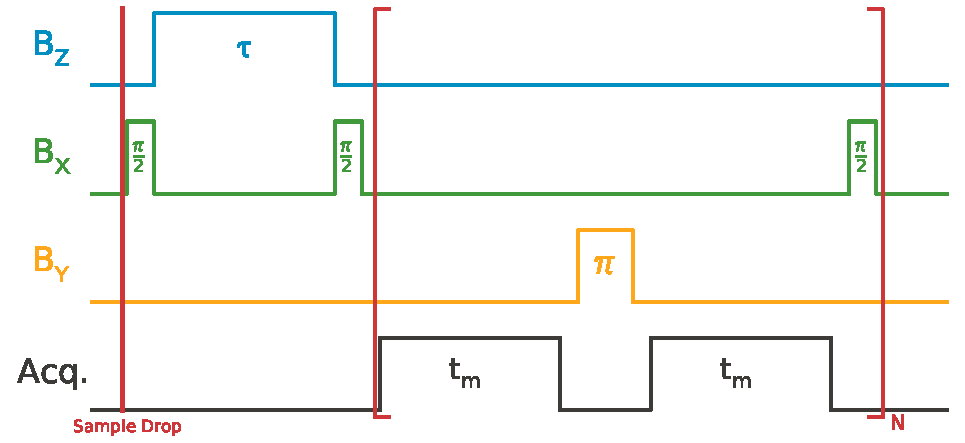
\includegraphics[width=\tw]{figures/relaxometry/quad_fid_acq_sequence_diagram.pdf}
\caption{A sequence for acquiring quadrature magnetization signals.}
\label{fig:QuadraturePulseSequence}
\end{figure}

This sequence causes the signal along $\vec{z}$ to alternate between representing the $\vec{x}$ and $\vec{y}$ components of the precession in the indirect dimension, such that the real channel ($\vec{x}$) signal is given by $l_{4n+2}-l_{4n+1}$ and the imaginary channel ($\vec{y}$) signal is given by $l_{4n+4}-l_{4n+3}$ where $l_n$ is the average signal level in the $n^{\textrm{th}}$ lobe of the square wave, and $n = [0, \sfrac{(N-1)}{4}]$ for $N$ lobe. Assuming that you start with your magnetization entirely in the $\vec{x}-\vec{z}$ plane (though this is more likely to be generated by rotating spins by $\sfrac{\pi}{2}$ along $\vec{y}$ after some evolution in the $\vec{x}-\vec{y}$ plane), a train of $\pi_{x}-\sfrac{\pi}{2}_{y}$ pulses is applied at a fixed interval. For a given initial density matrix:

\begin{equation}
\label{eqn:QuadDensityMatrixInit}
\rho_{0} = c_{z}I_{z} + c_{x}I_{x}
\end{equation}

The values of $c_{z}$ and $c_{x}$ are the real and imaginary components of the signal, respectively. The initial $\pi_{x}$ pulse has no effect on the $I_{x}$ spins, but flips the $I_{z}$ spins, giving a difference of $2c_{z}$. After a $\sfrac{\pi}{2}_{y}$ pulse, the $\vec{z}$ component is tipped to be along $\vec{x}$, and the $\vec{x}$ component is tipped to be along $\vec{z}$, giving:

\begin{equation*}
\rho = c_{z}I_{x} - c_{x}I_{z}
\end{equation*}

Flipping these spins with a $\pi_{x}$ pulse gives a difference of $-2c_{x}$, and after one more $\sfrac{\pi}{2}_{y}$ pulse, the initial density matrix from Eqn. \ref{eqn:QuadDensityMatrixInit} is restored and the pulse cycle can be repeated indefinitely. One concern with this sequence is that there's an asymmetry between the real and imaginary channels due to decay in the direct dimension. If distortions arise, it is likely preferable to switch to a 2-transient acquisition mode, where the measurement is repeated twice, once measuring the real channel and the other measuring the imaginary channel. If, for some reason, this is undesirable but 2 transients can still be used (for example, in the case where data is being analyzed initially in real time with transients repeated somewhat infrequently), then it is likely worthwhile to phase cycle the sequence. 

This is done by alternating the detected magnetization between being in the $\vec{x}-\vec{z}$ and $\vec{y}-\vec{z}$ plane, where in the first case the pulse sequence is $\left(\pi_{x}-\sfrac{\pi}{2}_{y}\right)_{n}$ (with initial pulse $\sfrac{\pi}{2}_{x}$ if the spins need to be rotated from the $\vec{x}-\vec{y}$ plane), and in the second case the pulse sequence is $\left(\pi_{y}-\sfrac{\pi}{2}_{x}\right)$ (with initial pulse $\sfrac{\pi}{2}_{y}$ if the spins need to be rotated from the $\vec{x}-\vec{y}$ plane). Alternatively, the sequence can be phase cycled without alternating between detection in the $\vec{x}-\vec{z}$ plane and $\vec{y}-\vec{z}$ plane by simply switching the order of the pulses between $\left(\pi_{x}-\sfrac{\pi}{2}_{y}\right)$ and $\left(\sfrac{\pi}{2}_{y}-\pi_{x}\right)$. When the first pulse is a $\pi$ pulse, it should come \textit{after} the first lobe of the square wave, whereas when the first pulse is a $\sfrac{\pi}{2}$ pulse, it should come \textit{before} the first lobe of the square wave. In both phase cycling methods, there are asymmetries between the two phases - method 1 (alternating between $\vec{x}-\vec{z}$ and $\vec{y}-\vec{z}$) has greater symmetry in the number of pulses applied and the type of pulses (e.g. lobe 2 always follows a $\pi$ pulse, lobe 3 always follows a $\sfrac{\pi}{2}$ pulse, etc), whereas method 2 has greater symmetry in the pulse directions (e.g. all $\sfrac{\pi}{2}$ pulses are all along $\vec{x}$), and greater symmetry in the coordinate system (e.g. the components of the spin polarization are always constrained to the $\vec{x}-\vec{z}$ plane). In most cases, the two methods will have identical outcomes, and they should only be important in systems which have some particular inhomogeneities or pulse imperfections.

\begin{figure}[ht!]
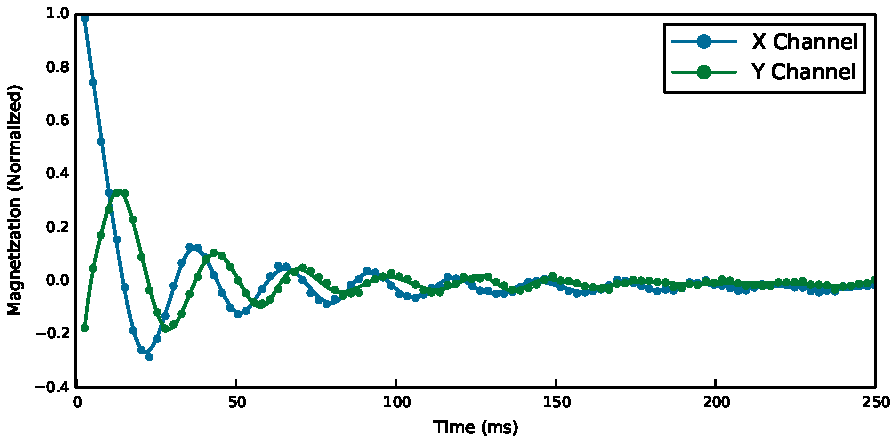
\includegraphics[width=\tw]{figures/relaxometry/quadrature_fid_data.pdf}
\label{fig:QuadratureDetectedFID}
\caption{An FID acquired with the quadrature detection sequence.}
\end{figure}

\subsection{Vector Signal Detection}
\label{nmr.signal.magnetization.vector}
The more generalized form of the quadrature detection scheme is a method for detecting the full vector spin polarization along all three components, using largely the same principles as those used in the quadrature detection. Because NMR precession usually occurs in a single plane, it is very unlikely that a vector detection sequence of this sort would be needed. It is most likely to be useful in the case of a sample after it has been passed through an unknown field, or when attempting to determine the direction of arbitrary offset fields.

As in the quadrature pulse sequence, the sequence is an alternating train of $\pi$ and $\sfrac{\pi}{2}$ pulses along $\vec{x}$ and $\vec{y}$. Using a ``pulse-conservative'' approach, wherein every pulse applied switches between measurement states, it is not possible to return to the original state after cycling through the pulses once, as the cycle results in a shift of an  odd permutation (e.g. xyz $\rightarrow$ yzx or zyx), which cannot be reversed with a single $\tfrac{\pi}{2}$ pulse. However, repeating the same cycle twice (e.g. x$\rightarrow$y$\rightarrow$z$\rightarrow$x$\rightarrow$y$\rightarrow$z) returns to the original permutation state (up to a phase). The simplest pulse sequence which accomplishes this, in general form, is:

\begin{equation}
\label{eqn:VectorPulseGeneralForm}
\left(\tau_m-\pi_{\tbinom{x}{y}}-\tau_m-\tfrac{\pi}{2}_{\pm\varphi}-\tau_m-\pi_{\tbinom{x}{y}}-\tau_m-\tfrac{\pi}{2}_{\pm\bar{\varphi}}\right)_{3n}
\end{equation}

In Eqn. \ref{eqn:VectorPulseGeneralForm}, $\varphi$ is either $x$ or $y$. At each point in this subsequence, a binary choice is presented, either choosing between $x$ or $y$, or choosing between $+\varphi$ and $-\varphi$ (or $\pm\bar{\varphi}$, as applicable). These choices affect only the sign of the outputs along each vector, while the choice of $\varphi$ determines the permutation order of the outputs. The pulses transform the inputs (keeping track of phase) as in \ref{eqn:RotationCoordinateTransforms}.

\begin{equation}
\label{eqn:RotationCoordinateTransforms}
\begin{aligned}
&       & \specialcell{\hfill{}\pi_{\tbinom{x}{y}}\hfill{}}          &           &\hspace*{7.5mm}&       & \specialcell{\hfill{}\tfrac{\pi}{2}_{x}\hfill{}}           &        &\hspace*{7.5mm}&       & \specialcell{\hfill{}\tfrac{\pi}{2}_{y}\hfill{}}           &        & \\                                      
& I_{x} & \xrightarrow{\hspace*{15mm}} & \pm I_{x} && I_{x} & \xrightarrow{\hspace*{15mm}} & \phantom{-}I_{x}  && I_{x} & \xrightarrow{\hspace*{15mm}} & -I_{z} & \\
& I_{y} & \xrightarrow{\hspace*{15mm}} & \mp I_{y} && I_{y} & \xrightarrow{\hspace*{15mm}} & \phantom{-}I_{z}  && I_{y} & \xrightarrow{\hspace*{15mm}} & \phantom{-}I_{y}  & \\
& I_{z} & \xrightarrow{\hspace*{15mm}} & -I_{z}    && I_{z} & \xrightarrow{\hspace*{15mm}} & -I_{y} && I_{z} & \xrightarrow{\hspace*{15mm}} & \phantom{-}I_{x}  & 
\end{aligned}
\end{equation}

From this, we can determine the phase of each output (necessary for consistent data processing) and choose a sequence of pulse phases which returns the spins to their original state after 12 pulses. Assigning boolean values $\mathbf{A}$-$\mathbf{D}$ to the binary choices presented in Eqn. \ref{eqn:VectorPulseGeneralForm}, the resulting states, \ref{eqn:VectorSequenceCyclePhiX} and \ref{eqn:VectorSequenceCyclePhiY} are: 

\begin{equation}
\begin{aligned}
&       &\hspace*{5mm}&               &\hspace*{5mm}&               &\hspace*{5mm}&        &\hspace*{5mm}&       & \\
&       && \specialcell{\hfill{}\mathbf{A}\hfill{}}   &&     \specialcell{\hfill{}\mathbf{B}\hfill{}}             && \specialcell{\hfill{}\mathbf{C}\hfill{}}     &&        \specialcell{\hfill{}\mathbf{D}\hfill{}}         & \\
&I_{x}: && \overset{x}{\tbinom{+}{-}} && \overset{x}{\tbinom{+}{+}} && \overset{x}{\tbinom{+}{-}}  && \overset{z}{\tbinom{-}{+}}& \\
&I_{y}: && \overset{y}{\tbinom{-}{+}} && \overset{z}{\tbinom{+}{-}} && \overset{z}{\tbinom{-}{-}}  && \overset{x}{\tbinom{+}{-}}& \\
&I_{z}: && \overset{z}{\tbinom{-}{-}} && \overset{y}{\tbinom{-}{+}} && \overset{y}{\tbinom{-}{+}}  && \overset{y}{\tbinom{+}{+}}&
\end{aligned}
\label{eqn:VectorSequenceCyclePhiX}
\tag{$\varphi = x$}
\end{equation}

\begin{equation}
\begin{aligned}
&       &\hspace*{5mm}&               &\hspace*{5mm}&               &\hspace*{5mm}&        &\hspace*{5mm}&       & \\
&       && \specialcell{\hfill{}\mathbf{A}\hfill{}}   &&     \specialcell{\hfill{}\mathbf{B}\hfill{}}             && \specialcell{\hfill{}\mathbf{C}\hfill{}}     &&        \specialcell{\hfill{}\mathbf{D}\hfill{}}         & \\
&I_{x}: && \overset{x}{\tbinom{+}{-}} && \overset{z}{\tbinom{-}{+}} && \overset{x}{\tbinom{+}{-}}  && \overset{z}{\tbinom{-}{+}}& \\
&I_{y}: && \overset{y}{\tbinom{-}{+}} && \overset{z}{\tbinom{+}{-}} && \overset{z}{\tbinom{-}{-}}  && \overset{x}{\tbinom{+}{-}}& \\
&I_{z}: && \overset{z}{\tbinom{-}{-}} && \overset{y}{\tbinom{-}{+}} && \overset{y}{\tbinom{-}{+}}  && \overset{y}{\tbinom{+}{+}}&
\end{aligned}
\label{eqn:VectorSequenceCyclePhiY}
\tag{$\varphi = y$}
\end{equation}

Taking ``true'' to result in a phase of $-1$ and ``false'' to result in a phase of $1$, and where a boolean ``true'' chooses the top choice (e.g. if $\mathbf{A}$ is true, the first pulse is $\pi_{x}$, otherwise $\pi_{y}$, if $\mathbf{B}$ is true, the second pulse is $\tfrac{\pi}{2}{+\phi}$, etc) the state after a single application of the minimum subsequence unit is given as:

\begin{equation}
\label{eqn:VectorSequenceCycleLogicalUnits}
\begin{aligned}
&            && \specialcell{\hfill{}\varphi = x\hfill{}} &&                                         &\hspace*{15mm}&             && \specialcell{\hfill{}\varphi = y\hfill{}} &&                                           &\\
& c_{x}I_{x} && \xrightarrow{\hspace*{10mm}}              && \neg\mathbf{ACD}\left(c_{x}I_{z}\right) &              & c_{x}I_{x}  && \xrightarrow{\hspace*{10mm}}              &&  \neg\mathbf{ABD}\left(c_{x}I_{y}\right)  &\\
& c_{y}I_{y} && \xrightarrow{\hspace*{10mm}}              && \mathbf{ABD}\left(c_{y}I_{x}\right)     &              & c_{y}I_{y}  && \xrightarrow{\hspace*{10mm}}              &&  \mathbf{ACD}\left(c_{y}I_{z}\right)      &\\
& c_{z}I_{z} && \xrightarrow{\hspace*{10mm}}              && \neg\mathbf{BC}\left(c_{z}I_{y}\right)  &              & c_{z}I_{z}  && \xrightarrow{\hspace*{10mm}}              && \neg\mathbf{BC}\left(c_{z}I_{x}\right)    &
\end{aligned}
\end{equation}

Repeating the sequence 3 times (with $\varphi$ constant) cycles through all 3 states, and so if $\mathbf{A}$, $\mathbf{B}$, $\mathbf{C}$ and $\mathbf{D}$ are kept constant, all three axes accumulate the same phase, which is given by Eqns. \ref{eqn:VectorSequencePhaseAccumulationX} and \ref{eqn:VectorSequencePhaseAccumulationY}:

\begin{equation}
\label{eqn:VectorSequencePhaseAccumulationX}
\neg\mathbf{ABC}\oplus\mathbf{ABD}\oplus\neg\mathbf{BC} = 0
\end{equation}

\begin{equation}
\label{eqn:VectorSequencePhaseAccumulationY}
\neg\mathbf{ABD}\oplus\mathbf{ACD}\oplus\neg\mathbf{BC} = 0
\end{equation}

In both cases, the phase cancels out, and the spins return to their original state with no phase, so long as $\mathbf{A}$, $\mathbf{B}$, $\mathbf{C}$ and $\mathbf{D}$ are constant throughout. It then only remains to determine which lobes correspond to which axial measurements - and what phase do these have. In the $\varphi = x$ sequence, these are given by Eqns. \ref{eqn:VectorSequenceLobesX} ($\varphi = x$) and \ref{eqn:VectorSequenceLobesY} ($\varphi = y$): 

\begin{equation}
\label{eqn:VectorSequenceLobesX}
\begin{aligned}
 2c_{x} & = \neg\mathbf{ACD}\left(l_{12n+4}-l_{12n+5}\right), \neg\mathbf{D}\left(l_{12n+10}-l_{12n+11}\right) && \\
 2c_{y} & = \neg\mathbf{AB}\left(l_{12n+2}-l_{12n+3}\right), \neg\mathbf{BC}\left(l_{12n+8}-l_{12n+9}\right) && \\
 2c_{z} & = \left(l_{12n}-l_{12n+1}\right), \mathbf{AC}\left(l_{12n+6}-l_{12n+7}\right) && 
\end{aligned}
\end{equation}

\begin{equation}
\label{eqn:VectorSequenceLobesY}
\begin{aligned}
 2c_{x} & = \neg\mathbf{AB}\left(l_{12n+2}-l_{12n+3}\right), \neg\mathbf{BC}\left(l_{12n+8}-l_{12n+9}\right) && \\
 2c_{y} & = \mathbf{ACD}\left(l_{12n+4}-l_{12n+5}\right), \mathbf{D}\left(l_{12n+10}-l_{12n+11}\right) && \\
 2c_{z} & = \left(l_{12n}-l_{12n+1}\right), \mathbf{AC}\left(l_{12n+6}-l_{12n+7}\right) && 
\end{aligned}
\end{equation}


Here $l_i$ is the magnitude of $I_{z}$ at lobe $i$, for $i \in [0, N]$ where N is the total number of pulses applied. These can be grouped more easily if it is assured that the two measurements of each axis always have the same phase, as this reduces the minimum number of lobes in the repeating sequence. Since the phase accumulated between any two measurements is always $\mathbf{AC}$ in both $\varphi = x$ and $\varphi = y$, this condition is met so long as $\mathbf{A} = \mathbf{C}$. Although we're likely indifferent to the individual phases, for symmetry we can also choose to constrain the phases to always be positive by choosing $\mathbf{B} = \neg\mathbf{A}$ and $\mathbf{D} = 1$ in the case of $\varphi = x$, and $\mathbf{B} = \neg\mathbf{A}$, $\mathbf{D} = 0$ in the case of $\varphi = y$. With these constraints, the vector form is given by:

\begin{equation}
\label{eqn:VectorSequenceLobes}
\begin{aligned}
 2c_{\varphi} &= l_{6n+2}-l_{6n+3} & \\
 2c_{\bar{\varphi}} &= l_{6n+4}-l_{6n+5} & \\
 2c_{z} &= l_{6n}-l_{6n+1} &
\end{aligned}
\end{equation}

As was the case in the quadrature detection scheme, since these lobes are separated in time by several $\tau$, $\tau$ should likely be chosen such that $\tau \ll T_{2}$. If asymmetry between the channels is a problem, phase cycling between the $\varphi=x$ and $\varphi=y$ sequences may be somewhat helpful. If a 3-phase cycle is needed (i.e. $x$-first, $y$-first then $z$-first), it is likely better to make three separate scalar measurements of $c_{x}$, $c_{y}$ and $c_{z}$, rather than a single vector measurement, as this will give much less distortion.

\section{Indirect Detection and Field Cycling}
\label{nmr.indirect}
Many experiments can be more easily performed in an indirect dimension by measuring changes in the sample magnetization (or in some cases, the spectrum) as a function of changes in some experimental parameter. The use of an indirect dimension is also particularly useful when the experiment is best performed in a magnetic field other than the detection field - such experiments are performed in a field cycled indirect dimension, wherein a field is applied during the experiment period which is removed during detection.

One simple example of a field cycled experiment is the detection of a free-induction decay curve along an indirect dimension. These signals can be time-consuming to acquire, and may as a consequence have poor spectral resolution, but they are often very useful for characterizing something about the sample (see Sec. \ref{nmr.gradcal}) or the coils used to apply the bias field (see Sec. \ref{nmr.pulsecal.FID}). The pulse sequence for an FID measurement is found in Fig. \ref{fig:FIDIndirectPulseSequence}.

\begin{figure}[ht!]
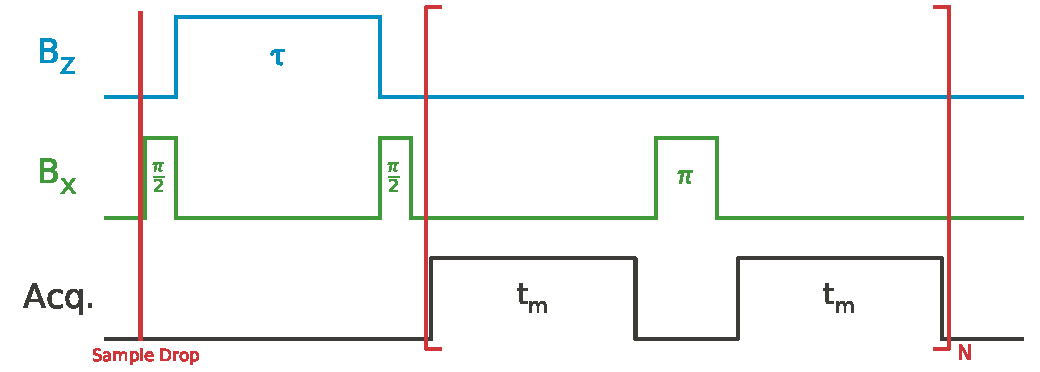
\includegraphics[width=0.95\tw]{figures/relaxometry/fid_acq_sequence_diagram.pdf}
\caption{The pulse sequence for a free-induction decay measurement along a field-cycled indirect dimension.}
\label{fig:FIDIndirectPulseSequence}
\end{figure}

The sample is prepolarized, and upon being dropped, the spins are pointing along $\vec{z}$, so a $\tfrac{\pi}{2}$ pulse is applied to tip them into the transverse plane. After the spins are tipped into the transverse plane, a field along $\vec{z}$ is applied for time $\tau$, after which time a second $\tfrac{\pi}{2}$ pulse tips the spins along $\vec{z}$, after which one of the magnetization detection pulse sequences is applied (See Sec. \ref{nmr.signal.magnetization}) for more details), and the magnetization is plotted as $\tau$ is varied. The result of one such measurement (real channel only) is shown in Fig. \ref{fig:FIDIndirectResult}.

These measurements are much more time consuming than detection in a direct dimension, as nearly the entire experiment needs to be repeated for each point in the experiment - which means waiting at least $3T_{1}$ for the sample to polarize, and in the case of prepolarized samples, adding twice the shuttling / transport time to the experimental time. In the case of magnetometers, it is possible to shift the detection frequency such that the detection is on-resonance at higher fields, allowing the experiments to be performed in a direct dimension - however, this eliminates much of the versatility of a zero-field detection scheme. Any time the magnetometer detection frequency is shifted, it will need to be calibrated at the higher field, and the pulse frequency and power will have to adjusted to match. In the indirect detection scheme, however, the bias field during the experiment can be varied arbitrarily and the magnetometer need not be re-calibrated. Additionally, the bias field is removed while the DC rotation pulses are applied, and so the pulses can be used without re-calibration at any experiment field. 


\begin{figure}[ht!]
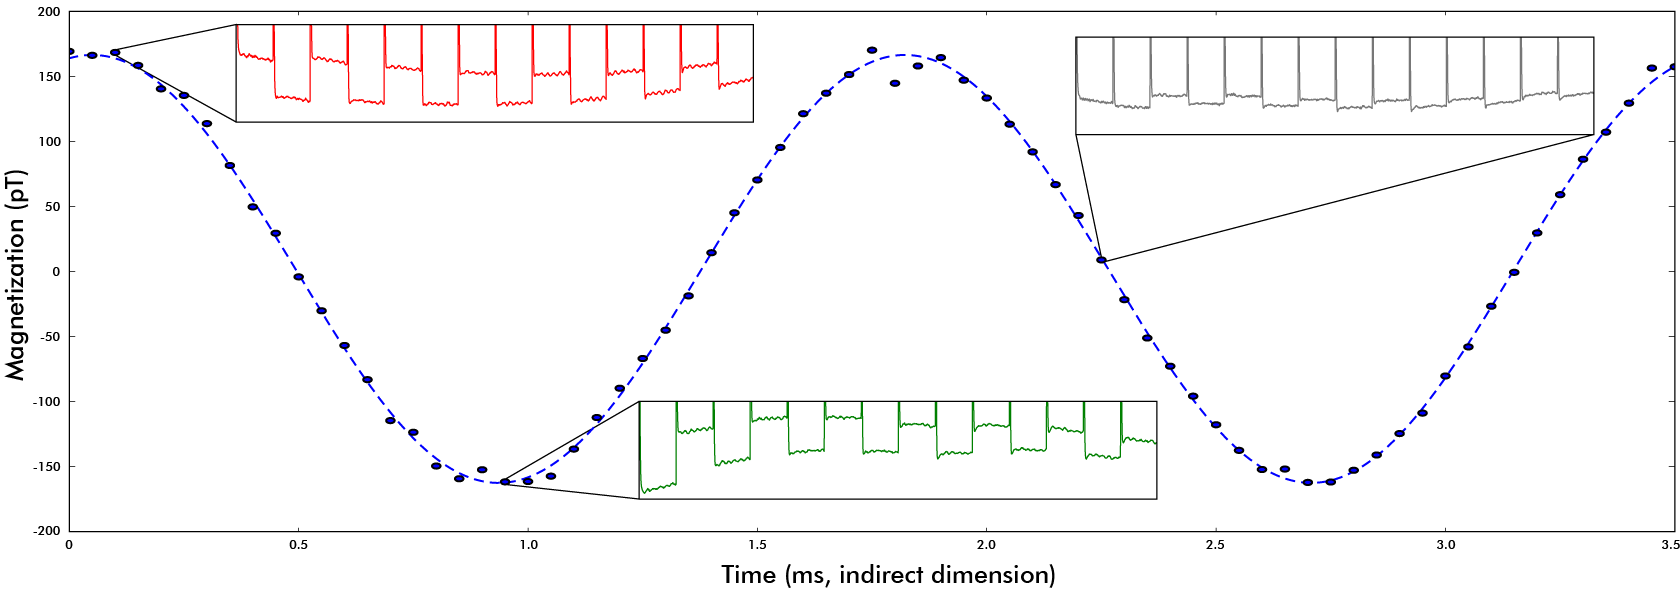
\includegraphics[width=\tw]{figures/relaxometry/12-07-17-WaterFID.png}
\caption{A free-induction decay curve acquired in an indirect dimension, field cycled to \unit[139]{mG}}
\label{fig:FIDIndirectResult}
\end{figure}

A sort of middle-ground between pure direct dimension detection and detection in an indirect dimension is the use of a windowed acquisition sequence. In such sequences, the experiment proceeds in the direct dimension, but is interrupted periodically for short periods to apply a brief measurement sequence. This allows the entire experiment to be acquired in a single transient in the direct dimension, but there is some trade-off between spending more time making measurements (increasing the signal-to-noise), making more measurements (increasing the resolution), and allowing the experiment to proceed without distortions from the field cycling. While these are some cause for concern, the greatest challenge in making windowed acquisition work is the dead time of the magnetometer. After a pulse is applied, the magnetometer signal becomes saturated, and so no measurements can be made until the alkali spins have had time to become polarized again (which depends on the pumping rate) - this is often on the order of \unit[10-30]{ms}, while the pulses are on the order of \unit[100]{$\mu s$}. The loss of \unit[10-30]{ms} per pulse necessitates measurement times ($\tau_m$) on the order of \unit[50]{ms} per lobe, and so a single magnetization measurement can take up a significant fraction of the entire experiment time (which is often on the order of a few seconds). With a faster re-polarization time, it would, however, be possible to do many of these experiments in a windowed direct dimension.

\section{Pulse Strength Calibration}
\label{nmr.pulsecal}
In order to know how long to apply pulses for, it's important to know the calibration of the pulse coils. This value depends on many factors - the coil configuration, the pulse circuit, the sample position and the nuclear gyromagnetic ratio, to name a few. For some of the more complicated pulse sequences, errors in these calibrations can become very important, as hundreds of pulses may be applied, or the signal may be very sensitive to small errors in the pulse length. As such, it is very important to have robust methods for finding the right pulse calibration.

\subsection{Calculated}
\label{nmr.pulsecal.calculation}
While calculations of the pulse strength will not necessarily provide low-error pulse calibration values, as they only address the idealized form of the coil geometry, they can make an excellent first-order approximation for what length you can expect from a given coil configuration. These sort of electromagnetic simulations can also give some insight into some aspects of the coil which may be difficult to estimate experimentally, such as the pulse inhomogeneity over the sample volume. 

Using the same Biot-Savart law simulator used to generate the homogeneity assessments in Fig. \ref{fig:PulseCoilHomogeneityComparisonFFT}, the strength and homogeneity of pulses in the region of interest (the sample), the expected FID for evolution under a given pulse can be calculated, and from the frequency of oscillation, the pulse lengths can be extracted. Since the input to the pulse coils is a voltage, but the coil response is a function of amperage, it is also necessary to simulate the pulse coil circuit to determine the correspondence between voltage in and current across the coil, this is one of the most likely sources of error in the calculation, as it may significantly depend on potentially hard-to-measure properties of the circuit components.

The calculated $\pi$ pulse times for the x, y, and z coils using the standard \unit[5]{V} input pulses are predicted from this approach as $t_{x,s}$ = \unit[95.8]{$\mu$s}, $t_{y,s}$ = \unit[90.4]{$\mu$s} and $t_{z,s}$ = \unit[153.3]{$\mu$s}\footnote{Here the ``s'' subscript denotes simulated results, while ``e'' represents experimental results.}, with the differences arising because of differences in the size, resistances and inductances of the coils. When measured with the multipulse method described in Sec. \ref{nmr.pulsecal.multiplepulse}, the $\pi$ pulse times are determined to be $t_{+x,e}$ = \unit[92.56]{$\mu$s}, $t_{-x,e}$ = \unit[87.15]{$\mu$s}, $t_{+y,e}$ = \unit[92.8]{$\mu$s} and $t_{-y,e}$ = \unit[87.15]{$\mu$}; the $\sfrac{\pi}{2}$ pulse length for the positive 90 channel was similarly measured at \unit[47.3]{$\mu$s}. Using the sample FID method described in Sec. \ref{nmr.pulsecal.FID}, the z coil's response was determined to be \unitfrac[0.14]{G}{V}, which corresponds to a \unit[5]{V} pulse time of \unit[167.5]{$\mu$s}.

As expected, the calculated pulse times are roughly correct, in all cases within $\pm$\unit[10]{\%} of the correct values. The fact that the negative pulses are stronger than the positive pulses may be a coincidence, or may be due to a systematic difference -- it is potentially the result of differences between the NPN and PNP transistors used in the amplification stage of the pulse coil; since the coils themselves are passive components, it seems unlikely that there is any systematic difference between current flowing in different directions across them. There is also a difference between the effective coil response between the $\pi$ and $\sfrac{\pi}{2}$ pulses, with the $\sfrac{\pi}{2}$ pulse taking somewhat more than half as long as the $\pi$ pulse. This is most likely explained by the effect of rise time in the coil, which is a decreasing fraction of the pulse as a function of time. An alternative explanation for this difference would be some sort of heating effect in components of the circuit, but this seems unlikely, because the experimental investigation reveals that the pulse time is not effected by duty cycle, as long as the time between pulses is longer than the ringdown time. Because the SPICE simulator does simulate the transient response of the circuit and coil, if more accurate calculations are required, it would be possible to incorporate this information into the model.

\subsection{Sample FID}
\label{nmr.pulsecal.FID}
A fairly accurate, but time-consuming way of measuring pulse length can be found by measuring the sample's free-induction decay (FID) as it evolves under the field produced by the pulse coil. Sample FID offers two primary advantages over other methods of pulse strength calibration. The first advantage is that the shape of an FID can give information about the homogeneity of the pulse and also the effects of the pulses' rise and fall times. Pulse distortions are likely to be greatest for very small $t_{p}$, whereas these distortions will average out over the course of a longer pulse. Additionally, by taking longer-term measurements (likely since these detections occur in an indirect dimension, these should be heavily aliased to reduce the number of samples), the FID curves and/or the Fourier transform spectra can be used to determine $T_{2}^*$ (the inhomogeneous broadening from the pulse coil).

 As such, while the pulse angle should be linear in the duration of the pulse (and, as such, fitting to 2-3 points should be enough to calibrate pulses of arbitrary angle), the true signal may be have a non-linear response, particularly for short pulses. Likely the best way to characterize the nature of this non-linearity is by taking a sample FID, which measures the angular frequency response as a function of pulse duration. This also relates to the second advantage, which is that the FID simultaneously measures the pulse time for a wide array of angles, whereas the much more commonly used Pulse Train method (Sec. \ref{nmr.pulsecal.pulsetrain}) is only used to calibrate for a single pulse angle (though, very accurately).

The data are acquired in an indirect dimension, and since they use magnetization detection, require that the pulses already be somewhat calibrated (poorly calibrated pulses will cause aliased precession in the direct dimension, leading to reduced magnetization signal, though the FID can certainly still be detected without issue), as such, it is likely best to use the multiphase $\pi$ train described in Sec. \ref{nmr.signal.magnetization.pitrain}, as this can reduce pulse-related errors.

\subsection{Pulse Train}
\label{nmr.pulsecal.pulsetrain}
The most common and in many cases the best way to calibrate the strength of the pulse strength is by applying a train of the pulses to a sample and observing the results. Unlike the sample FID method, which can give a decently accurate prediction of the length of a pulse of arbitrary angle, pulse train measurements can be used to determine the pulse length of a pulse of a specific angle to nearly arbitrary precision - in most cases the pulse calibration will be limited by the clock speed of the pulse generator, not by uncertainty in the calibration process itself. That said, depending on the number of pulses to be calibrated (usually it's best to start with at least 4: $\pi_{x}$, $\pi_{y}$, $\tfrac{\pi}{2}_{x}$ and $\tfrac{\pi}{2}_{y}$) and the degree of accuracy, this can also become quite time consuming.

The pulse train experiment should generally be designed like a magnetization detection experiment where the pulse time is varied over some plausible range. For calibrating pulses $\theta \neq n\pi$, it is preferable to repeat the pulse $n$ times where $n = \tfrac{m\pi}{\theta}$ where $m$ is an odd number - under this condition, the magnetization should be inverted after each pulse when the appropriate pulse time calibration has been found. Caution should be taken to leave a sufficiently long space between pulses to allow the coil to fully discharge, otherwise the fact that multiple pulses are being applied in a row will affect the calibration, and an error can be introduced. Generally the appropriate inter-pulse spacing can be found by repeating the same experiment a few times with different inter-pulse spacings to gauge the magnitude of the effect.

Such a pulse-acquire-pulse-acquire sequence is equivalent to making a measurement in the direct dimension of the spin precessesion under the pulse - and choosing pulses close to the duration of a $\pi$ pulse is equivalent to sampling such that the signal precession is the same as the Nyquist frequency - which should alias the signal down to \unit[0]{Hz}, and any precession that occurs is indicative of either a pulse error or a bias field (see Sec. \ref{nmr.pulsecal.multiplepulse} for more details on how to deal with a bias offset). For a candidate pulse $t_{c} = t_{\pi} + t_{\varepsilon}$, where $t_{\pi}$ is the optimal $\pi$ pulse length and $t_{\varepsilon}$ is the error in the pulse length, the resulting signal should effectively oscillate at frequency $\omega_{\varepsilon} = \gamma B_{0} \sfrac{t_{\varepsilon}}{\tau_{m}}$. Because relaxation occurs during the $\tau_{m}$ period as well as during the pulses, the linewidth depends on both choice of $t_{c}$ and $\tau_{m}$. The magnetization decay and precession after 1 $t_{c}$ pulse and 1 $\tau_{m}$ measurement period, assuming that $T_{2}^*$ is roughly constant, is given by Eqn. \ref{eqn:PulseCalibrationTrainEvolution}:

\begin{equation}
\label{eqn:PulseCalibrationTrainEvolution}
M_{1} = M_{0}e^{-\tfrac{t_{c}\left(1 + \sfrac{\tau_{m}}{t_{c}}\right)}{T_{2}^*}}e^{-i\gamma B_{1}t_{c}}
\end{equation}

As such, the effective $T_{2}^*$ of the measurement is $T_{2p}^* = \sfrac{T_{2}^*}{(1+\tfrac{\tau_{m}}{t_{c}})}$, and the observed linewidth will be $\sfrac{(1+\tfrac{\tau_{m}}{t_{c}})}{\pi T_{2}^*}$. This essentially limits the accuracy of such measurements to $\omega_{\varepsilon} < T_{2p}^*$, as slow precession on the timescale of relaxation is very difficult to accurately measure. However, this is really a somewhat ``soft'' limit on the error, as more pulses can be applied before another measurement is taken - switching from a train of $\pi$ + $\varepsilon$ to $3\pi + 3\varepsilon$ will give a signal precessing at effectively 3 $\omega_{\varepsilon}$, and so the pulse error can be reduced by a factor of just under 3. Longer trains of pulses will, of course, increase $t_{c}$ relative to $\tau_{m}$, and a maximum is reached when $t_{c} = \sfrac{\tau_{m}T_{2C}^*}{T_{2M}^*}$, where $T_{2C}^*$ is the $T_{2}^*$ during the $t_{c}$ pulse and $T_{2M}^*$ is the $T_{2}^*$ during the measurement. This value can easily be less than the limiting condition where the period of the pulse generator's clock is less than $\gamma t_{\varepsilon} B_{1}$ , since at that point uncertainty is limited by the ability to pulse accurately. It is not worth increasing the accuracy of $t_{c}$ beyond this point, as the pulses cannot be applied with sufficient precision anyway.

\subsubsection{Multiple Pulse Method}
\label{nmr.pulsecal.multiplepulse}
The major problem with the pulse train method is that it cannot distinguish between a small error in the pulse time and an uncorrected bias offset field along the direction of the pulse. While some bias offsets can be removed using the applied oscillation method (see. Sec. \ref{mag.design.shim.coils.zeroing.oscillation}), the vector signal is sensitive to light shifts along the direction of the pump and probe beams, and so the field which ``zeros'' the magnetometer signal along those directions is in fact applying a real magnetic field that the sample spins will feel to counter an effective magnetic field that they will not. The effective frequency as a function of $t_{c}$ is then given by Eqn. \ref{eqn:PulseCalSignalWithBias}:

\begin{equation}
\label{eqn:PulseCalSignalWithBias}
\omega = \gamma B_{1}t_{\varepsilon} + \gamma B_{r}\left(t_{c} + \tau_{m}\right),
\end{equation}

where $B_{r}$ is the residual bias field. One way to solve this problem is to keep $t_{c}$ constant and measure $\omega$ as a function of $\tau_{m}$. The slope of this line should be $\gamma B_\epsilon$, which can be zeroed out and the experiment repeated until the slope is constant. This can also be done empirically, by varying $\tau_m$ in the direct dimension and varying the bias offset field until there is no precession during any value of $\tau_{m}$ - if this is to be done, it is best to switch $\tau_{m}$ only after an even number of equal-sized lobes, as this largely retains the spin-echo properties of the $\pi$ train, whereas alternating each lobe between multiple values of $\tau_{m}$ hampers echo formation, and so fields along the two other orthogonal dimensions must be simultaneously corrected as well.

This method may work for zeroing the field, but then the pulse error becomes tied to the precision of the shim coils. This may not be problematic, but a much more accurate pulse calibration method - which works largely independent of the bias offset field - is to perform the pulse train calibration multiple times, varying the number of $\pi$ pulses applied before each measurement. The signal after $N$ pulses is

\begin{equation}
\label{eqn:MagSignalAfterNPulses}
M_{N} = (-1)^{N}e^{-\sfrac{Nt_{c}}{T_{2C}^*}}e^{-iN\gamma B_{1}(t_{\varepsilon}) - i\gamma B_{\epsilon}t_{c}}.
\end{equation}

As can be seen from Eqn. \ref{eqn:MagSignalAfterNPulses}, the pulse error $t_{\varepsilon}$ is a function of $N$, but the evolution under the bias offset field is not. As such, in a measurement of $\omega$ as a function of $t_{c}$ and $N$, the $t_{c}$ at which all values of $\omega_{N}$ intersect is the point where $t_{\varepsilon}$. Once this is found, it can be used to zero field as detailed in Sec. \ref{mag.design.shim.coils.zeroing.sample.nmr} on the NMR sample precession field zeroing method.

\section{Gradient Strength Calibration}
\label{nmr.gradcal}
\begin{figure}[ht!]
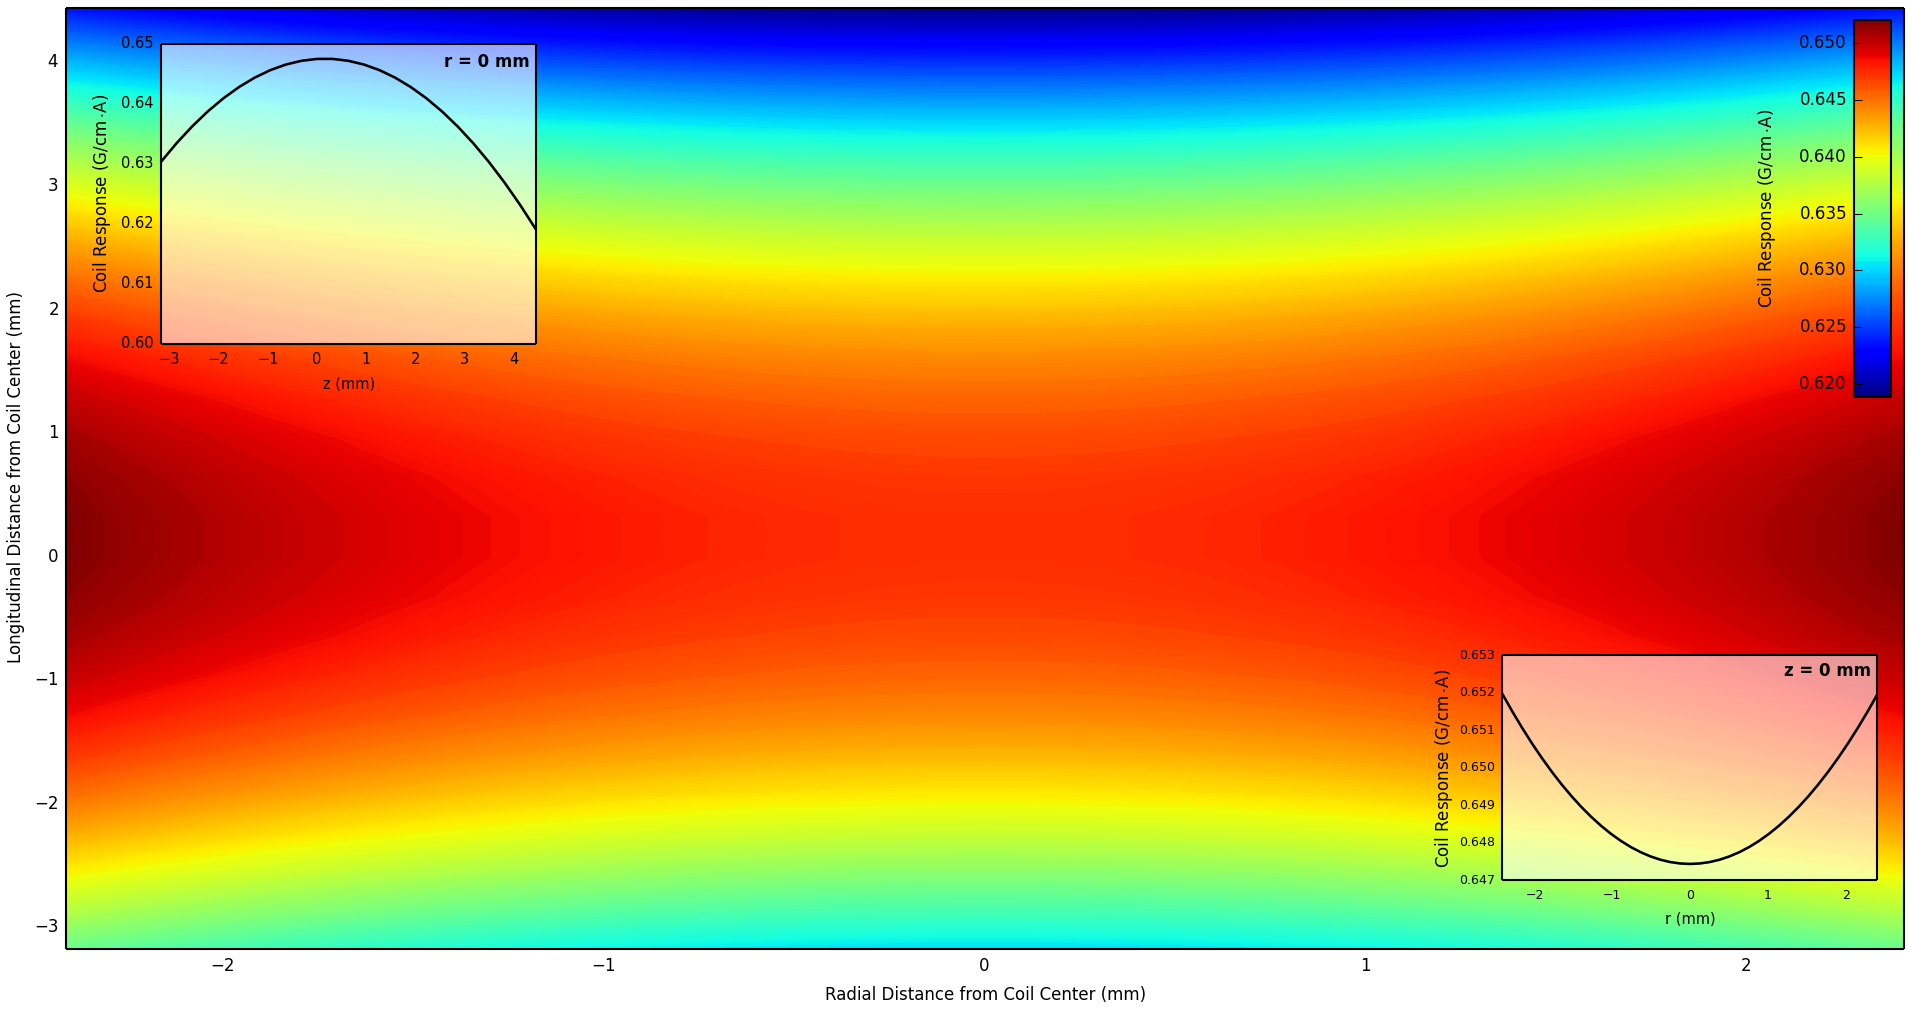
\includegraphics[width=\tw]{figures/coils/GradientMap.png}
\caption{A contour map of the calculated gradient field generated in the region of the sample by the anti-Helmholtz pair used in the diffusion experiments. Inset at the top left is a projection of the gradient strength along the longitudinal axis, and inset at the bottom right is a projection along the radial axis.}
\label{fig:GradientMap}
\end{figure}
The accuracy of diffusion (and imaging) experiments depends on having an accurate calibration of the strength of the magnetic field. Since the gradient strength is set by the analog voltage outputs, it depends both on the response of the coils and the coefficient of the voltage-to-current DC pulse circuit, described in Sec. \ref{pulse.circuit}. As with the pulse coils, this can be determined to first order from electromagnetic calculations, but this many not adequately capture deviations from ideality in the pulse coil or circuit. 

The coils are centered \unit[0.125]{"} (\unit[0.3175]{cm}) above the top of the heater; the thickness of the probe head cap at its thinnest is \unit[0.0125]{"} (\unit[0.03175]{cm}), and the NMR tube glass is \unit[0.38]{mm} thick, so the lowest sample position is \unit[0.098]{"} (\unit[2.478]{mm}) below the center of the gradient. The results of Biot-Savart law calculations for the anti-Helmholtz pair in this region are shown in Fig. \ref{fig:GradientMap}. The weighted average value of the gradient in this region is \unitfrac[0.64]{G}{cm$\cdot$A}, with no more than \unit[0.4]{\%} deviation within this volume.

\begin{figure}[ht!]
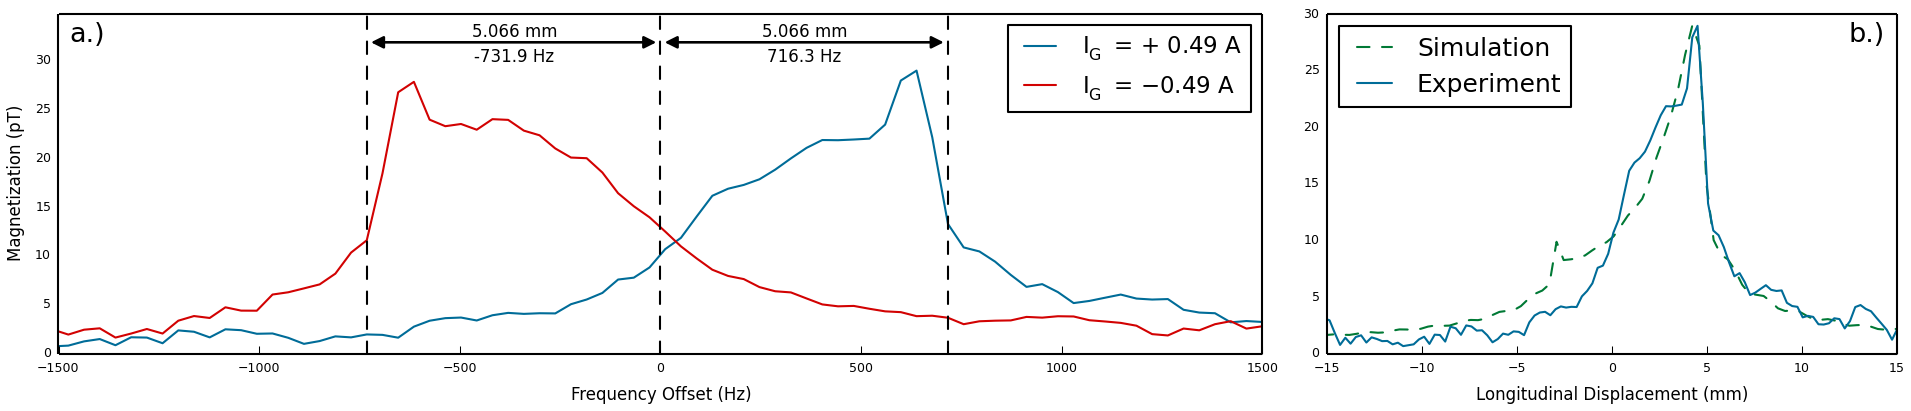
\includegraphics[width=\tw]{figures/coils/GradientImage.png}
\caption{a.) An image taken of a sample \unit[5]{mm} NMR tube filled with \unit[100]{$\mu$L} of water while applying a \unit[0.5]{G} bias offset field and \unit[$\pm$0.49]{A} across the gradient coil. b.) The lineshape is compared to one calculated from a Biot-Savart simulator taking into account the simulated gradient, sample volume and beam intersection volume.}
\label{fig:GradientImage}
\end{figure}

Likely the best way to confirm the gradient strength is to take an image (1-dimensional) with known dimensions and determine the gradient strength from the correspondence between frequency and position,

\begin{equation}
\Delta x = \frac{\Delta f}{2\pi\gamma G},
\label{eqn:FrequencyPosition}
\end{equation}

which can be arranged to solve for $G$ as such:

\begin{equation}
G = \frac{\Delta f}{2\pi\gamma\Delta x}.
\end{equation}

Ideally, a phantom with distinct features of known size varying across its length would be used to displace sample, effectively allowing individual gradient measurements along the entire volume of the phantom. Due to time pressure and the difficulty of constructing a phantom that would stay in place while being shuttled, this approach was not feasible, so instead an image was taken of a sample of known volume (\unit[100]{$\mu$L}) using both the positive and negative gradient coils, and a small bias offset (\unit[0.5]{G}) intended to truncate concomitant gradients. Inverting Eqn. \ref{eqn:VolumeAnyTube} (introduced in a more thorough discussion of sample volumes in Sec. \ref{Section:Relaxation-Diffusion-Hydrocarbons-Mixtures-PhysicalSeparation}), and confirmed by measurement with a micrometer, this corresponded to a height of \unit[7.88]{mm}. Because the gradient coils are centered \unit[2.478]{mm} above the bottom of the sample, there should be a precipitious drop-off in signal \unit[5.07]{mm} from the center frequency of the FID. The results, based on an FID with 201 points sampled in an indirect dimension at \unit[20]{kHz} are shown in Fig. \ref{fig:GradientImage}. The result was that the positive gradient calibration was found to be \unitfrac[0.68]{G}{cm$\cdot$A} and the negative gradient calibration was found to be \unitfrac[0.69]{G}{cm$\cdot$A}\footnote{The reason these are different is likely because of differences in the circuitry. Since the pulse controller uses a voltage-controlled current source, in reality, the gradient calibrations were calculated to be \unitfrac[0.0443]{G}{cm$\cdot$V} and \unitfrac[0.0452]{cm$\cdot$V}, respectively, but this cannot be compared directly with the Biot-Savart calculations without an analysis of the circuit.}

\section{Sample Temperature}
\label{nmr.sampletemp}
Because the cell  operates at elevated temperature, even with active air cooling the NMR samples are often somewhere above room temperature - and with liquid nitrogen-based cooling they may in fact be below room temperature. Many effects, important among them being relaxation and diffusion, depend strongly on temperature, and this should be accounted for when analyzing data. However, making direct measurements of the sample temperature in situ can be quite problematic - the sample needs to be able to move, and so a thermocouple cannot be inserted directly into it for monitoring, many layers of the instrumentation must be opaque, and so optical monitoring of the temperature is problematic, and because the sample is both actively being air-cooled and shuttled, the equilibrium temperature of the sample will depend, to some extent, on the rate of equilibration and the duty cycle (up vs. down). 

Generally to combat the effect of sample heating over the course of an experiment, experiments were designed such that either the duty cycle did not change over the course of the experiment, though in some situations this was not necessarily possible and may have introduced small drifts in the signal into the samples. The biggest observed temperature change artifact was generally during the first few transient acquisitions, after the sample had been allowed to reach thermal equilibrium at room temperature, and was thus took a few transients to reach a new thermal equilibrium. To combat this, generally the sample was run through several ``dummy'' experiments, wherein no data are acquired before starting the real experiment. Generally pulses were still applied in these experiments, in case any of the pulse components were similarly undergoing heating which might change their effective coil response.

Without active liquid N$_{\mathrm{2}}$ cooling (described in more detail in \Cref{nmr.pneumatic.sample}), typical temperatures observed were on the order of \unit[35-37]{\degsym C}, and with no air-cooling, the system tended to equilibrate closer to \unit[60]{\degsym C}.

\subsection{Relaxation-based Measurement Method}
\label{nmr.sampletemp.relaxation}
The easiest and most robust way of measuring temperature --- which we use as a standard in our experiments --- is by using a calibrated NMR relaxation signal. Water relaxation, in particular, is extremely sensitive to temperature, and so by measuring a calibration curve of temperature vs. NMR relaxation constants, water from the same source (relaxation is also highly dependent on impurities) can be used as a standard thermometer. Unfortunately, for the same reason that it is not possible to continuously monitor the temperature of the samples, the instrument itself could not be used to make these calibration measurements, and so a Magritek Terranova-MRI Earth's field NMR system was used to make standard calibration curves. Because water's $\mathrm{T}_{1}$ and $\mathrm{T}_{2}$ are also quite sensitive to magnetic field at low fields, all relaxation-based temperature measurements made in the magnetometer were field-cycled to \unit[0.435]{G}, which was the field in which the Terranova experiments were performed.\footnote{The Terranova system has two T$_1$ measurement sequences, measuring ``B$_P$'' and ``B$_E$'', B$_P$ measures T$_1$ recovery in the Terranova's prepolarizing field, while B$_E$ measures T$_1$ decay in Earth's field.} The results are summarized in Table \ref{Table:T1T2DataTempTerranova}.

\begin{table}[h]
\centering
\tabulinesep=1.5mm
\begin{tabu} spread 0.65\tw {X[1.5,m,l]X[m,c]X[m,c]} \hline
Temp. (\degsym C)   & T$_1$ (s)         &   T$_2$ (s)  \\ \hline
27  &  2.5 &  2.24 \\ 
39  &  3.5 &  3.19 \\ 
54  &  4.5 &  4.9  \\ 
64  &  5.7 &  6.2  \\ 
84  &  7.8 &  6.7  \\ \hline
\end{tabu}
\caption{The T$_1$ and T$_2$ measurements of DI water from UC Berkeley's Stanley Hall, performed at \unit[0.435]{G}.}
\label{Table:T1T2DataTempTerranova}
\end{table}

To make these measurements, a special sample bottle was prepared, a glass bottle insulated with several layers of fiberglass insulation. The bottle had two caps, one unmodified cap to be used during the measurements, and a second cap with a thermocouple inserted through a hole and held in place with epoxy. The second cap was used to monitor the temperature between experiments. The water was boiled in a standard electric tea kettle and poured into the glass bottle, then allowed to cool to room temperature over the course of several hours. As cooling processes follow an exponential decay, there is more uncertainty in the highest temperatures - the reported temperatures are an average of the temperature measured immediately before and after the experiment. This is not an ideal way to perform this experiment, as the temperature uncertainty is compounded by the fact that water's T$_1$ is inversely proportional to temperature, thus necessitating long experiments at the highest temperatures (which are cooling the fastest). An experiment with active temperature control of the sample would be much more accurate.

The standard model for the temperature dependence is a bi-exponential rate equation of the form:\cite{Simpson1958,Hindman1973,bentum-2011}

\begin{equation}
\frac{1}{T_1} = A_{1}e^{-\sfrac{E_{1}}{RT}} + A_{2}e^{-\sfrac{E_{2}}{RT}}.
\label{eqn:T1TemperatureEquation}
\end{equation}

From the somewhat sparse data in Table \ref{Table:T1T2DataTempTerranova}, fitting the data gives $A_{1}$ = \unit[1.303$\cdot 10^{-4}$]{s}, $A_{2}$ = \unit[8.49$\cdot 10^{-4}$]{s}, $E_{1}$ = \unitfrac[44.5]{kJ}{mol}, $E_{2}$ = \unit[14.9]{kJ}{mol}, which are generally consistent with literature values measured at higher fields.

\section{Detectable Sample Region and Sample Geometry}
\label{Section:NMR-Detectable-Region}
Unlike in a traditional NMR spectrometer or a SQUID magnetometer, where the sample sits entirely within the detector volume, atomic magnetometers are inherently one-sided \textit{ex-situ} devices which measure the magnetic field generated by the region surrounding the detector. Additionally, in a simple one-detector setup, the detection efficiency dies off as $\sfrac{1}{r^3}$ where $r$ is distance from the detector. Generally, the size of the most sensitive region of the magnetometer is proportional to the size of the detector - which in practice means (approximately) the intersection volume of the beams within the cell.

Additionally, the geometry of the NMR sample tubes is such that the most sensitive region (the bottom of the tube) is curved, losing signal where it is most important and somewhat complicating the signal profile. Assuming the curved bottom of the NMR tube is approximately hemispherical, the lost detection volume is $\tfrac{1}{3}\pi r^3$ where $r$ is the radius of the tube, which for a \unit[5]{mm} diameter NMR tube with \unit[0.381]{mm} wall thickness is $\approx$ \unit[9.96]{$\mu L$}. Generally, signal closer to the signal is much stronger than signal far from the detector. The signal at the origin from a dipole $\vec{\mu}$ at $\vec{r}$ is given by

\begin{equation}
\label{eqn:FieldFromADipole}
B(\vec{r}) = \frac{\mu_0}{4\pi}\frac{(\vec{\mu}\cdot\vec{r})\vec{r} - \left|\vec{r}\right|^2\vec{\mu}}{\left|\vec{r}\right|^5}.
\end{equation}

The $\vec{z}$ component of this volume is 
\begin{equation}
\label{eqn:ZFieldFromADipole}
B_z(\vec{r}) = \frac{\mu_0\mu_z}{4\pi}\frac{3\cos^2(\varphi)-1}{|\vec{r}|}.
\end{equation}

Eqn. \ref{eqn:ZFieldFromADipole} is positive inside a cone with angle $\theta_{m}$, where $\theta_{m}$ is the magic angle, $\theta_{m} = \cos^{-1}(\sfrac{1}{\sqrt{3}}) \approx $\unit[54.7356]{\degsym} and negative outside that cone. In general, picking out the positive lobe of a cone defined by $\varphi_0$, the signal from a magnetized volume gives

\begin{equation}
\label{eqn:FieldFromVolume}
\int_{0}^{R}\int_{0}^{\pi}\int_{-\varphi_{0}}^{\varphi_{0}}\frac{3\cos^2(\varphi)-1}{r^3}\mathrm{d}\varphi\sin(\theta)\mathrm{d}\theta r^2\mathrm{d}r = 2\log(R)\left[\varphi_0 + \tfrac{3}{2}\sin(2\varphi_{0})\right].
\end{equation}

The area inside the $\theta_{m}$ cone contributes $2\log(R)\left[2\theta_{m} + \sqrt{2}\right]$ to the signal, and the remaining area on the positive lobe ($-\tfrac{\pi}{2} \leq \varphi \leq \tfrac{\pi}{2}$) contributes $\pi - 2\theta_{m} - \sqrt{2}$, which is $\approx$ 32.6\% of the maximum signal. 

 Additionally, curved surfaces are much stronger than flat surfaces in response to impact (for one thing, the surface area of a hemisphere is $4\pi r^2$, whereas for a flat surface, it's $2\pi r^2$, so in a curved surface, the force is distributed about twice as much area), and so the glass can be thinner as a result. It is likely an empirical question what thickness tubes will be usable, and depends on many factors.
\end{document}